% -------------------- DON'T EDIT ----------------------------------------
\documentclass[a4paper,12pt,oneside,openany]{xepersian-thesis-iasbs-ftex}
\usepackage[top=3.5cm,right=3cm,bottom=4cm,left=3cm]{geometry}  
\usepackage{amsmath,amsfonts,amssymb,amsthm}
 \usepackage[marginal,stable,bottom]{footmisc}     % for footnotes: marginal --> the same margins as text, 
                                                                                  %                       stable--> ?
                                                                                  %                       bottom --> starting the footnotes at a fixed place at the bottom of the page.
 
%\usepackage{perpage}                                             % for footnotes: starting from 1 perpage
%\usepackage{zref-abspage}
%\zmakeperpage{footnote}
%\MakePerPage{footnote}
%added by samim zarrin pour : DO NOT UNCOMMENT ABOVE LINES (4)
\usepackage{zref-perpage}
\zmakeperpage{footnote} 

\usepackage{cite}                                                     % for collecting citations: [1,2,3,4] --> [1-4]
\usepackage{setspace}                                            % for switching between double/single space in document
\allowdisplaybreaks                                                    % breaking the lines&pages when needed for the style.
\usepackage{parskip}                                               % ? 

%\relpenalty=9999                                            % show the neccessity of breaks for lines, changing the number to 10000 cause no break in lines.
%\binoppenalty=9999

\usepackage{xecolour}
\usepackage{makeidx}
\usepackage{verbatim}
\usepackage[colorlinks,linkcolor=blue,citecolor=blue]{hyperref}
\usepackage{graphicx}
\usepackage{ifthen}

 \parindent0pt


\makeatletter
\pdfstringdefDisableCommands{%
\let\lr\@firstofone
}
\makeatother
% ----------------------------------------------------------------------------
%added by samim zarrin pour
%to include hyperlinks
\usepackage{hyperref}
%to highlight freefem++ code
\usepackage{ff++listings}
%for figures
\usepackage{caption}
\usepackage{subcaption}
%for R symbol
\usepackage{amssymb}
%for algorithms
\usepackage[]{algorithm2e}

\usepackage[extrafootnotefeatures]{xepersian}

\usepackage[Lenny]{fncychap}

\settextfont[Scale=1.07]{XB Niloofar}
\setlatintextfont[Scale=1.05]{Times New Roman}
\setdigitfont[Scale=1.05]{Yas} 
% قلم برای اعداد به صورت فارسی با صفر توخالی، در صورتی که بخواهیم اعداد انگلیسی نوشته شوند این خط را غیر فعال می‌کنیم.

\defpersianfont\nastaliq[Scale=2.0]{IranNastaliq}
% قلم برای نوشتن تقدیم
\defpersianfont\nastaliqone[Scale=1.0]{IranNastaliq}
% قلم نستعلیق با سایز متناسب با متن در صورت نیاز
\defpersianfont\anotherfont[Scale=1.2]{XP Ziba}
% قلم برای نوشتن تشکر (قلم فانتزی)
\newenvironment{fantezi}
{\anotherfont }


\makeindex


\def\beginto{
\newpage
\begin{RTL}
\begin{Huge}
\nastaliq

\begin{center}
\vspace*{0.15cm}
تقدیم به 
}

\def\endto{
~
\end{center}
\end{Huge}
\end{RTL}
}

\def\beginthanks{
\newpage

{\centering\Huge{\nastaliqone{
تشکر وقدردانی ~\\
~\\}}}
}

\def\endthanks{
~
}

\def\thanks{
\beginthanks
پس از تشکر از فداکاری‌های خانواده عزیزم و حمایت‌های مستمرشان لازم می‌دانم از دکتر هاشم صابر نجفی عزیز  به خاطر هدایت بنده به سمت مدل‌سازی و ریاضی کاربردی و استاد راهنمای صبورم، دکتر خدیجه ندائی اصل به خاطر حمایت‌های علمی و درک بسیار بالای ایشان تشکر کنم. و از هرچه بگذربم سخن دوست خوش‌تر است ...



\endthanks
}

\def\startpage{
\newpage
\vspace*{3cm}
\begin{center}

\includegraphics[width=12cm]{besm}
\end{center}
}
\makeatletter
\def\@makechapterhead#1{%
  \vspace*{50\p@}%
  {\parindent \z@ \centering\normalfont
    \ifnum \c@secnumdepth >\m@ne
      \if@mainmatter
        \huge\bfseries \@chapapp\space \tartibi{chapter} 
        \par\nobreak
        \vskip 20\p@
      \fi
    \fi
    \interlinepenalty\@M
    \Huge \bfseries #1\par\nobreak
    \vskip 40\p@
  }}
\def\@makeschapterhead#1{%
  \vspace*{50\p@}%
  {\parindent \z@ \centering
    \normalfont
    \interlinepenalty\@M
    \Huge \bfseries  #1\par\nobreak
    \vskip 40\p@
  }}
\makeatother



\renewcommand\bibname{مراجع}
\def\contentsname{فهرست}

% some extra diffinitions %%%%%%%%%%%%%%%%%
%%%%%%%%%%%%%%%%%%%%%%%%%%%%%

\def\bea{\begin{eqnarray}}
\def\eea{\end{eqnarray}}

\def\ba{\begin{array}}
\def\ea{\end{array}}

\def\ni{\noindent}
\def\nn{\nonumber}

\def\bc{\begin{center}}
\def\ec{\end{center}}




\usepackage{afterpage}
\usepackage{amsmath,mleftright}
\usepackage{amsthm}
\usepackage{mathrsfs}
\usepackage{amssymb}

\newcommand\blankpage{%
	\null
	\thispagestyle{empty}%
	\addtocounter{page}{-1}%
	\newpage}
% ------------------- You Can EDIT ----------------------------------------
\graphicspath{
	{chap1_images/}
	{chap2_images/}
	{chap3_images/}
	{images/}
}                       % The paths to the images.

% -------------------- DON'T EDIT ----------------------------------------

\begin{document}
\lstset{language=freefem++}
% -------------------- PLEASE EDIT ---------------------------------------

% --------------------------------------   INFORMATION IN PERSIAN  ---------------------------------------

\title{حل عددي معادلات ديفرانسيل با مشتقات جزئی با ضرايب نامعين به کمک شبکه عصبی}
\author{ساجد زرین پور نشرودکلی}
%--------------------------------------------
% از بین دو حالت زیر یکی را فعال کنید:
\degree{کارشناسی ارشد ریاضیات کاربردی - آنالیز عددی}
%\degree{دکتری}
%---------------------------------------------
\supervisor{دکتر خدیجه ندائی اصل}
% در صورتی که استاد مشاور داشته‌اید نام وی را در خط زیر بنویسید در غیر این صورت خط زیر باید غیرفعال باشد.
\advisor{دکتر پروین رزاقی}\advisorexisttrue
\department{دانشکده علوم ریاضی}
\university{دانشگاه تحصیلات تکمیلی در علوم پایه زنجان}
\city{زنجان}
\thesisdate{شهریور ۱۳۹۹}
\makepersiantitle
% -------------------------------------------------------------------------------------------------------------------
%\startpage
% -------------------------------------------------------------------------------------------------------------------

%\beginto
%%در اینجا پایان‌نامه خود را به هر کس که دوست دارید تقدیم کنید. در غیر این صورت این قسمت را غیر فعال کنید.
%%آنان که زبان طبیعت را برای توصیف طبیعت می‌جویند.
%\endto
% -------------------------------------------------------------------------------------------------------------------
%اگر در فایل thanks از دوستان و همکاران خود تشکر کرده‌اید خط زیر را فعال کنید، در غیر این صورت این خط باید غیرفعال باشد.
%\thanks
% -------------------------------------------------------------------------------------------------------------------
\newpage
\begin{abstract}
\addcontentsline{toc}{section}{چکیده} % To add the abstract in the index.
برای مدل‌سازی پدیده‌های واقعی با معادلات دیفرانسیل با مشتقات جزئی که شامل عدم قطعیت است، یکی از مشکلات وجود مجموعه‌ای از پدیده‌ها است که به عنوان مشکلات ابعاد بالا شناخته می‌شوند. خوشبختانه، اغلب تغییرات متغییرهای مدل می‌توانند توسط تعداد کمی خصوصیات دامنه توسط روش‌های کاهش مدل، ثبت شوند. برای مثال، می‌توان با استفاده از روش‌های مبتنی بر شبکه‌های عصبی متغییرهای مورد نظر را به عنوان تابعی از ضرایب ورودی اندازه‌گیری کرد. در این‌صورت، نمایش پذیری متغیرها توسط چنین شبکه‌ای را می‌توان با دید شبکه عصبی به عنوان یک تحول زمانی برای پیداکردن جواب‌های مدل توجیه کرد. در این پایان نامه، ما یک روش میانبر برای پیدا کردن جواب‌های مدل روی دو معادله دیفرانسیل با مشتقات جزئی معروف در فیزیک و مهندسی را بازبینی مینمائیم. همچنین، ما به سراغ بررسی یک روش عددی سنتی از نظر تئوری خواهیم رفت و از این طریق، احتمالات جدیدی برای استفاده از شبکه‌های عصبی در حل معادلات دیفرانسیل را مطرح خواهیم نمود.
%مدلسازي بيشتر مسايل فيزيک به معادلات ديفرانسيل همراه با ضرايب عدم قطعيت منتهي مي‌شوند، به عبارت ديگر معادلاتي با ضرايب تصادفي. در بيشتر موارد اين عدم قطعيت مشتق شده از معادلات ديفرانسيل را مي‌توان با تعدادي از ويژگي‌هاي ميدان ضرايب کنترل کرد. بر همين اساس، پيشنهاد ما استفاده از يک روش بر پايه شبکه‌هاي عصبي براي پارامتري کردن کميت‌هاي فيزيکي مورد نظر به عنوان تابعي از ضرايب ورودي است.
%نمايش کميت مورد نظر با استفاده از شبکه عصبي مي‌تواند با ديد شبکه عصبي به عنوان تکامل دهنده در طي زمان براي پيدا کردن جواب‌هاي معادله ديفرانسيل با مشتقات جزئي تعديل شود. 

%دو معادله ديفرانسيل با کاربرد گسترده در فيزيک و مهندسي را مورد بررسي قرار مي‌دهيم که عبارت‌اند از معادله لاپلاس و معادله شرودينگر غيرخطي.
%معادلات بيضوي عموماً براي مطالعه‌ي اعمال گرماي يکنواخت روي يک ماده دلخواه به کار مي‌روند. زماني که ماده ناهمگن باشد(که با استفاده از ضرايب تصادفي در معادله بيضوي مدل مي‌شوند)، معمولاً به دنبال يافتن انتقال دماي موثر ماده هستيم.

%معادله شرودينگر غيرخطي براي يافتن انتشار نور در موج‌بر و همچنين در پديده‌هاي مکانيک کوانتومي که ذرات بوزونيک در پايين‌ترين حالت انرژي متمرکز شده‌اند (چگالش بوز-انيشتين) به کار مي‌رود. ما به دنبال يافتن جواب اين پرسش هستيم که انرژي چنين حالت اساسي‌اي وقتي معادله شرودينگر غيرخطي در مورد ميدان پتانسيل تصادفي مطرح شود چگونه رفتار خواهد کرد.
%براي سادگي در هر دو معادله ديفرانسيل، شرط مرزي، به طور متناوب در نظر گرفته شده است. مباحث عددي مورد نظر در اين پايان نامه مبتني بر روش تفاضل متناهي و روش شبکه هاي عصبي است.
%مدلسازي بيشتر مسائل فيزيک به معادلات ديفرانسيل همراه با ضرايب عدم قطعيت به عبارت ديگر معادلاتي با ضرايب تصادفي منتهي مي‌شوند.  در بيشتر موارد اين عدم قطعيت مشتق شده از معادلات ديفرانسيل را مي‌توان با تعدادي از ويژگي‌هاي ميدان ضرايب کنترل کرد. بر همين اساس، پيشنهاد ما استفاده از يک روش بر پايه شبکه‌هاي عصبي براي پارامتري کردن کميت‌هاي فيزيکي مورد نظر به عنوان تابعي از ضرايب ورودي است. نمايش کميت مورد نظر با استفاده از شبکه عصبي مي‌تواند با ديد شبکه عصبي به عنوان تکامل دهنده در طي زمان براي پيدا کردن جواب‌هاي معادله ديفرانسيل با مشتقات جزئي تعديل شود. 
%دو معادله ديفرانسيل با کاربرد گسترده در فيزيک و مهندسي را مورد بررسي قرار مي‌دهيم که عبارت‌اند از معادله لاپلاس و معادله شرودينگر غيرخطي.\\
%معادلات بيضوي عموماً براي مطالعه‌ي اعمال گرماي يکنواخت روي يک ماده دلخواه به کار مي‌روند. زماني که ماده ناهمگن باشد(که با استفاده از ضرايب تصادفي در معادله بيضوي مدل مي‌شوند)، معمولاً به دنبال يافتن انتقال دماي مؤثر ماده هستيم.
%معادله شرودينگر غيرخطي براي يافتن انتشار نور در موج‌بر و همچنين در پديده‌هاي مکانيک کوانتومي که ذرات بوزونيک در پايين‌ترين حالت انرژي متمرکز شده‌اند (چگالش بوز-انيشتين) به کار مي‌رود. ما به دنبال يافتن جواب اين پرسش هستيم که انرژي چنين حالت اساسي‌اي وقتي معادله شرودينگر غيرخطي در مورد ميدان پتانسيل تصادفي مطرح شود چگونه رفتار خواهد کرد.
%براي سادگي در هر دو معادله ديفرانسيل، شرط مرزي، به طور متناوب در نظر گرفته شده است. مباحث عددي مورد نظر در اين پايان نامه مبتني بر روش تفاضل متناهي و روش شبکه‌هاي عصبي است.
\keywords{شبکه‌های عصبی، روش تفاصلات متناهی، روش المان‌های متناهی، معادلات دیفرانسیل با مشتقات جزئی، عدم قطعیت.}

\end{abstract}
% -------------------------------------------------------------------------------------------------------------------

\tableofcontents
%\listoffigures
%\listoftables
\afterpage{\blankpage}

% -------------------------------------------------------------------------------------------------------------------

% اگر قبل از شروع فصل‌های پایان‌نامه مقدمه‌ای دارید، خط زیر را فعال کرده و مقدمه خود را در فایل introduction بنویسید. در غیر این صورت این خط باید غیر فعال باشد.
\newpage

\pagenumbering{arabic}\setcounter{page}{1}
%\vspace*{-1cm}
\pagenumbering{arabic}
\section*{Introduction}
\addcontentsline{toc}{section}{Introduction}

Here, I will write an introduction.

% ----------------------------------------   Chapters of the Thesis  ---------------------------------------------
\section*{مقدمه}
\addcontentsline{toc}{section}{مقدمه}
مقدارسنجی عدم قطعیت (۱۵) در فیزیک و مهندسی اغلب شامل مطالعه معادلات دیفرانسیل با مشتقات جزئی با میدان ضرایب تصادفی است. برای درک رفتار یک سیستم شامل عدم قطعیت، می‌توان کمیت‌های فیزیکی مشتق شده از معادلات دیفرانسیل توصیف کننده آن سیستم را به عنوان توابعی از میدان ضرایب استخراج کرد. اما حتی با گسسته‌سازی مناسب روی دامنه معادله و برد متغیرهای تصادفی، این کار به طور ضمنی به حل عددی معادله دیفرانسیل با مشتق جزئی به تعداد نمایی می‌انجامد.\\
یکی از روش‌های متداول برای مقدار سنجی عدم قطعیت، روش نمونه‌ برداری مونته کارلو است. گرچه این روش در بسیاری از موارد کاربردی است اما کمیت اندازه‌گیری شده ذاتاً دارای نویز است. به‌علاوه، این روش قادر به پیدا کردن جواب‌های جدید در صورتی که قبلا نمونه‌گیری نشده باشند، نیست. ما به‌دنبال یافت روشی هستیم که نویز داده‌ها در جواب آن تأثیر چندانی نداشته باشند و همچنین، قادر به ارائه جواب برای حالاتی که قبلا نمونه گیری نشده باشند نیز باشد. \\
روش گالرکین تصادفی با استفاده چند جمله‌ای‌های آشوب  یک جواب تصادفی را روی فضای متغیرهای تصادفی بسط می‌دهد و به این طریق مسئله با بعد بالا را به تعدادی معادله دیفرانسیل با مشتقات جزئی معین تبدیل می‌کند. این گونه روش‌ها به دقت زیادی درباره تعیین توزیع عدم قطعیت نیازمند هستند و از آن‌جا که پایه‌های استفاده شده مستقل از مسئله هستند، وقتی بعد متغیرهای تصادفی بالا باشد هزینه محاسباتی بسیار زیاد خواهد شد. ما به‌دنبال یافتن راهی برای حذف نیاز به محاسبه این پایه‌ها به صورت سنتی هستیم. یکی از اهداف این پایان‌نامه مطالعه نقطه ضعف روش‌های عددی سنتی همانند روش گالرکین تصادفی و روش المان‌های متناهی است. برای این منظور، تئوری روش المان‌های متناهی را مورد مطالعه دقیق‌تر قرار می‌دهیم.\\
هدف کار ما پارامتری کردن جواب یک معادله دیفرانسیل معین به کمک شبکه‌های عصبی (ساخت نمایشی دیگر برای جواب بر پایه ترکیب توابع) و سپس استفاده از روش‌های بهینه‌سازی برای یافتن جواب معادله است. در این پایان‌نامه تابع مورد نظر برای پارامتری‌سازی روی میدان ضرایب معادله دیفرانسیل با مشتقات جزئی تعریف شده است. در واقع ما به دنبال کاهش بعد مبتنی بر نمایش شبکه ‌عصبی برای حل معادلات دیفرانسیل با مشتقات جزئی همراه با عدم قطیت هستیم.
\section*{انگیزه و هدف}
\addcontentsline{toc}{section}{انگیزه و هدف}
مدل‌سازی طبیعت همیشه با پارامترهایی همراه است که مقادیر آنها از کنترل ما خارج است. اما عموما ما درباره محدوده تغییرات این پارامترها اطلاعاتی داریم. به معادلاتی که شامل این‌گونه پارامترها هستند، معادلات با ضرایب عدم قطعیت گوییم. به طور مثال، در مورد حرکت نفت در سفره‌های زیر زمینی؛ برای بیان شیوه حرکت مایعات نیاز به دانستن مکان حفره‌ها  در بافت سفره زیر زمینی داریم. این امر را می‌توان به صورت رسانایی مؤثر در حضور ناخالصی نیز در نظر گرفت. به عنوان مثالی دیگر، مسئله‌ای را مطرح می‌کنیم که نقطه شروع این رساله بوده است.\\ 
برای تشخیص سرطان پستان روش‌های متعددی موجود است. از جمله آن‌ها می‌توان به تصویر برداری پستان با بازتابش اشعه ایکس (XRM)\LTRfootnote{Projection X-ray mammography}، تصویربرداری با استفاده از ارتعاشات مغناطیسی (MRI)\LTRfootnote{Magnetic resonance imaging}، تصویربرداری فراصوت (US)\LTRfootnote{Ultra sound}، توموسنتز دیجیتال (DBT)\LTRfootnote{Digital breast tomosynthesis}، ماموگرافی انتشار پوزیترون (PET)\LTRfootnote{Positron emission mammography} و توموگرافی فراصوت (UST)\LTRfootnote{Ultra sound tomography} اشاره کرد. هرکدام از این روش‌ها اطلاعات را به طرق مختلفی نمایش می‌دهند، به این معنا که غده‌ای که در یکی از این روش‌ها غیر قابل تشخیص است در روش دیگر قابل تشخیص است؛ غده‌ای که در یک روش بافت مشکوک معرفی می‌شود، در روش دیگر می‌تواند به عنوان غده‌ای سالم و طبیعی معرفی شود. و این موضوع باعث ایجاد مشکلات بسیاری در روند تشخیص و برنامه ریزی درمان می‌شود. در این مرحله، راه‌حلی که به ذهن می‌رسد، ترکیب نتایج حاصل از این روش‌ها برای بالابردن ضریب دقت است؛ لیکن مشکل دیگری مانع این‌کار می‌شود. بافت پستان بسیار کشسان است و به راحتی تغییر فرم می‌دهد. از طرفی در هرکدام از این روش‌ها بیمار به حالت خاصی قرار می‌گیرد که با روش دیگر متفاوت است. به طور مثال، طی MRI بیمار در حالت دمر قرار دارد ولی برای تصویربرداری فراصوت بیمار به پشت می‌خوابد. علاوه‌براین، در روش بایوپسی راهنمایی شده توسط MRI\LTRfootnote{MRI-guided biopsy} بافت پستان توسط صفحه‌های سخت و غیرقابل انعطافی بی حرکت می‌شوند که منجر به فشرده شدن بافت نیز می‌شود. بنابراین، شکل، اندازه و مکان غده در این تصاویر متفاوت خواهد بود. این امر مقایسه تصاویر را با سختی بسیار همراه می‌کند. علاوه‌براین، برای برنامه‌ریزی پیش از جراحی، پزشک نیاز به دانستن مکان و اندازه دقیق غده دارد. بنابراین، نیاز به توسعه الگوریتم‌های ثبت غیرسخت\LTRfootnote{Non-rigid registration algorithm} احساس می‌شود.\\
روش‌هائی مبتنی بر روش المان‌های متناهی\LTRfootnote{Finite element method} برای حل این مسئله ارائه شده‌اند. اما مشکل عمده این روش‌ها هزینه محاسباتی بالای آنها است. مطابق آن‌چه در (۷) گفته شده است، به طور متوسط اجرای  یک شبیه‌سازی صد و بیست دقیقه به طول می‌انجامد که برای مصارف کلینیکی مقرون به صرفه نیست. مارتینز و همکارانش (۷) در سدد ارائه روشی برای کاهش این هزینه محاسباتی با استفاده از شبکه‌های عصبی بودند. گرچه، مدل ارائه شده توسط آنها زمان محاسبات را به طرز چشمگیری کاهش می‌دهد، اما پارامترهای مدل مورد مطالعه آن‌ها ثابت است. به عبارت دیگر، با توجه به این‌که این پارامترها از بدنی به بدن دیگر متفاوت هستند، برای ارائه یک مدل مختص به بیمار در زمانی قابل قبول، نیاز به توسعه مدل برای فراگیری پارامترهای دارای عدم قطعیت است. به طور مثال، نیازمند در نظر گرفتن ضریب کشسانی بدن بیمار، که یک ضریب عدم قطعیت است، هستیم. از این رو، برآن شدیم که بدنبال حل عددی معادلات دیفرانسیل (بیضوی) به کمک شبکه‌های عصبی باشیم.\\ 
%در این رساله، بدنبال حل عددی معادلات دیفرانسیل با مشتقات جزئی بیضوی خطی و غیر خطی ناهمگن هستیم. روشی که ما در صدد گزارش آن هستیم، یک روش کاهش بعد برای محاسبه جواب بدون نیاز به حل مستقیم معادله دیفرانسیل است. به عبارت دیگر، در روش‌های عددی متدوال، فرد بدنبال پیدا کردن تقریبی از جواب در یک فضای متناهی یا غیر متناهی است که در حالت متناهی به صورت ترکیب خطی از پایه هایی نوشته می‌شوند که در روند روش روی نقاط رأسی بدست می‌آیند. ما به‌دنبال راهی برای حذف ساخت این پایه‌ها به کمک شبکه عصبی هستیم و به این وسیله در پی کاهش بعد فضای جواب با حفظ خصوصیات اصلی مورد نیاز خود در جواب هستیم. با توجه به اینکه نمایش جواب بدست آمده از شبکه‌های عصبی به صورت ترکیبی متناهی از توابع بدست می‌آید می‌توانیم با تعویض نمایش جواب از حالت خطی (روش‌های عددی متداول) با حالت غیر خطی (نمایش شبکه‌های عصبی) به این مهم دست یابیم. ایده، استفاده از شبکه‌های عصبی برای یادگیری نگاشتی از دامنه ضرایب عدم قطعیت به فضای جواب بر اساس مجموعه داده‌ای از قبل محاسبه شده است.
در روش‌های عددی متدوال، هدف یافتن تقریبی از جواب مدل در یک فضای متناهی یا غیر متناهی است که به صورت یک ترکیب خطی از پایه های آن فضا در نقاط رأسی بدست می‌آید. دقت این تقریب با تعداد نقاط رأسی به کار رفته رابطه مستقیم دارد. بنابراین، محاسبه تقریبی دقیق برای مسائل پیچیده روی دامنه‌های پیچیده، همچون محاسبه میزان تغییر فرم بافت پستان در اثر نیروهای وارده، به ناچار مستلزم استفاده از تعداد بسیار زیادی نقاط رأسی روی دامنه مدل می‌باشد که به طور مستقیم منجر به افزایش زمان محاسبه جواب مدل می‌شود. از این‌رو  با تکیه بر اصول شبکه‌های عصبی بدنبال راهی برای حذف نیاز به محاسبه مستقیم پایه‌های فضای تقریب روی نقاط رأسی با استفاده از روشی مبتنی بر کاهش بعد فضای جواب با حفظ خصوصیات اصلی مورد نیاز خود از جواب هستیم. با توجه به اینکه نمایش جواب بدست آمده از شبکه‌های عصبی به صورت ترکیبی متناهی از توابع است، می‌توانیم با تعویض نمایش جواب از حالت خطی (روش‌های عددی متداول) با حالت غیر خطی (نمایش شبکه‌های عصبی) به این مهم دست یابیم. ایده، استفاده از شبکه‌های عصبی برای یادگیری نگاشتی از دامنه ضرایب عدم قطعیت به فضای جواب بر اساس مجموعه داده‌ از قبل محاسبه شده است. به این ترتیب می‌توان گفت روشی که ما در صدد گزارش آن هستیم، یک روش کاهش بعد برای محاسبه جواب بدون نیاز به حل مستقیم معادله دیفرانسیل است. در این رساله، معادلات دیفرانسیل با مشتقات جزئی بیضوی خطی و غیر خطی ناهمگن را مورد بررسی قرار می‌دهیم. نکته حائز اهمیت این است که از آن‌جا که این روش، یک روش مبتنی بر داده است، نوع مدل (بیضوی، هذلولوی و یا سهموی) یا روش عددی استفاده شده برای نمونه‌گیری جواب و ایجاد پایگاه داده جدید، در آن تغییر چشمگیری ایجاد نمی‌نمایند. بنابراین، این روش برای هر سه نوع معادلات دیفرانسیل با مشتقات جزئی در هردو حالت همگن و ناهمگن قابل استفاده است. از طرف دیگر، از آنجا که ما از محاسبات تنسوری در لایه‌های این شبکه بهره می‌بریم، این مدل با کمترین میزان تغییرات قابل استفاده در ابعاد بالاتر نیز است. برای نمایش این ادعا، معادله اول را در یک بعد و معادله دوم را در دو بعد بررسی خواهیم کرد.
\section*{مقدارسنجی عدم قطعیت }
\addcontentsline{toc}{section}{مقدارسنجی عدم قطعیت }
مقدارسنجی عدم قطعیت مطالعه اعتمادپذیری نتیجه‌گیری علمی است. به عبارت دیگر به جای مطالعه درستی هر فرضیه به طور جزئی، به دنبال  مطالعه ارتباط بین فرضیات هستیم. سؤال اساسی در مسائل مقدار سنجی عدم قطعیت این است که با فرض اینکه اطلاعاتی درمورد خطا در ورودی‌های مدل در دسترس باشد، در مورد تغییرات در خروجی چه می‌توان گفت؟(۱۵) برای مقدار سنجی عدم قطعیت یک کمیت فیزیکی، یکی از راه‌ها پیدا کردن نگاشتی از فضای پارامترهای عدم قطعی در ورودی مدل به فضای خروجی مدل است. خوشبختانه این نگاشت‌ها عموما وابسته به تعداد محدودی 'خصیصه` هستند که می‌توان آنها را با تعداد محدودی نمونه‌برداری و حل مدل دیفرانسیلی به‌دست آورد.\\
عموما عدم قطیت ناشی از فرضیات ساختار مدل و یا مقدار وردی‌های آن است. در این پایان‌نامه، ما روی عدم قطعیت حاصل از عدم قطعیت روی ورودی‌های مدل تمرکز خواهیم کرد. عدم قطعیت روی داده‌های ورودی به چهاردسته پارامترهای تصادفی، میدان‌های تصادفی، نویز سفید و همبسته طبقه‌بندی می‌شود (۱۶). در مسئله یافتن ضریب رسانایی مؤثر پر محیط ناهمگون عدم قطعیت روی داده های ورودی از نوع پارامترهای تصادفی و در مسئله تعیین سطح انرژی حالت پایه با پتانسیل زمینه ناهمگون از نوع نویز سفید هستند. \\
اغلب مقدار خروجی مورد نظر ما مقداری است که از فراوری‌ داده‌های خروجی مدل اولیه حاصل می‌شود. دراین‌جا نیز، هدف ما در واقع کنترل عدم قطعیت خروجی ثانویه مدل است که از فراوری حاصل می‌شود. با فرض اینکه عدم قطعیت ورودی مدل با بردار $\bm{a}=(a_1,\dots,a_N)^T$ پارامتری شده باشد، جواب معادله علاوه بر ابعاد فضایی $\bm{x}$ و بعد زمان $\bm{t}$ به بردار پارامترهای رندوم $\bm{a}$ نیز وابسته است. بنابراین یک نمونه‌گیری از جواب می‌تواند به صورت $u(x,t;a)$ به ازای یک انتخاب مشخص از پارامترهای رندوم بیان شود. گرچه ما علاقه‌‌مند به بررسی هر کدام از این نمونه‌ها به طور مجزا نیستیم (۱۶). بنابراین ما پایگاه داده خود را بر همین اساس خواهیم ساخت. کنترل عدم قطعیت مقدار خروجی مطلوب معمولا مستلزم تکامل یک انتگرال چندگانه روی بردار پارامتری $\bm{a}$ است (۱۶). مدل مطرح شده در این پایان‌نامه، این تکامل و تقریب عددی جواب آن را به طور همزمان بر عهده دارد. بدین منظور، به جای تلاش برای یافت جواب مدل، در سدد یافت نگاشتی از پارامترهای تصادفی ورودی به خروجی پردازش شده مدل هستیم. دقت کنید که به همین دلیل، با اینکه ما روش خود را روی معادلات بیضوی بررسی کردیم، همین روش برای معادلات هذلولوی و سهموی نیز کاراست.
\section*{تعریف مسئله }
\addcontentsline{toc}{section}{تعریف مسئله}
در این پایان نامه، هدف ما بررسی یک مدل میانبر برای حل مسائل معادلات دیفرانسیل با مشتقات جزئی به کمک شبکه‌های عصبی است. به عبارت روشن‌تر یافتن نگاشتی از فضای عدم قطعیت مسئله به فضای جواب. مسائلی که در این رساله برای حل انتخاب شده اند از این جهت حائز اهمیت بوده‌اند که هر دو حالت خطی و غیر خطی، معادلات دیفرانسیل غیر همگن شامل عدم قطعیت را پوشش می‌دهند.
\subsection*{یافتن ضریب رسانایی مؤثر در محیط ناهمگون}
معادله اول، رسانایی مؤثر در یک جهت انتخاب شده درون یک محیط غیر همگون را توسط ضریب رسانش توصیف می‌کند. محیط غیر همگون، محیطی است که در آن خصوصیات مورد توجه در تمامی نقاط یکسان نیستد. این امر ممکن است به دلایلی همچون جنس‌های گوناگون مواد تشکیل دهنده یا چگالی های متفاوت مربوط باشد. فرض ما بر آن است که ضریب رسانایی ماده در جهات متفاوت یکسان نباشد و این ضریب را با $\bm{a}(x)$ نمایش می‌دهیم. این بردار از نمونه‌گیری توابعی به فرم زیر روی نقاط رأسی حاصل می‌شود:
\begin{equation}
	\mathscr{A} = \{a\in L^{\infty}([0,1]^d) | \lambda_{1} \geq a(x) \geq \lambda_{0} > 0 \},
\end{equation}
که در آن $\lambda_{0}$ و $\lambda_{1}$ اعداد ثابتی هستند.با فرض انتخاب یک جهت دلخواه ثابت $\xi \in \mathbb{R}^d$، میزان ضریب رسانش در آن جهت مطلوب است. به عبارت دقیق‌تر، جواب معادله زیر مد نظر است
\begin{equation*}
A_{\text{eff}}(\bm{a}) = \min_{u(x)} \int_{[0,1]^d} \bm{a}(x) ||\nabla u(x) + \xi||_{2}^{2} \mathrm{d}x.
\end{equation*}
این معادله با فرم دیفرانسیلی زیر هم‌ارز است. به عبارت دیگر، جواب مسئله بهنه‌سازی فوق در معادله دیفرانسل زیر سدق میکند و جواب معادله دیفرانسیل زیر نیز تابع هدف مسئله بهینه‌سازی فوق را بهینه می‌کند.
\begin{equation}
	-\nabla \cdot (a(x)(\nabla u(x)+\xi)) = 0 
\end{equation}
ازاین‌رو، با جای حل مسئله مینیم‌سازی، فرم مذکور را به کمک گسسته‌سازی زیر با گام $h=\frac{1}{n}$ حل می‌نماییم.
\begin{multline*}
	-\sum_{k=1}^{d} \frac{a_{i+\frac{1}{2}e_{k}} - a_{i-\frac{1}{2}e_{k}}}{h} \cdot \frac{u_{i+e_{k}} - u_{i}}{h} - \sum_{k=1}^{d} a_{i-\frac{1}{2} e_k}  \frac{u_{i+e_{k}} - 2 u_{i} + u_{i-e_{k}}}{h^2} - \sum_{k=1}^{d} \xi_k \frac{a_{i+\frac{1}{2}e_{k}} - a_{i-\frac{1}{2}e_{k}}}{h} \\
	= - \sum_{k=1}^{d} \frac{ a_{i+\frac{1}{2}e_{k}} u_{i+e_k} - a_{i+\frac{1}{2}e_{k}} u_i - a_{i-\frac{1}{2}e_{k}} u_{i+e_k} + a_{i-\frac{1}{2}e_{k}} u_i + a_{i-\frac{1}{2}e_{k}} u_{i+e_k} - 2 a_{i-\frac{1}{2}e_{k}} u_i + a_{i-\frac{1}{2}e_{k}} u_{i-e_k}}{h^2} \\ - \sum_{k=1}^{d} \xi_k \frac{a_{i+\frac{1}{2}e_{k}} - a_{i-\frac{1}{2}e_{k}}}{h} \\
	= - \sum_{k=1}^{d} \frac{ a_{i+\frac{1}{2}e_{k}} [u_{i+e_k} - u_i] -  a_{i-\frac{1}{2}e_{k}} [u_i - u_{i-e_k}]}{h^2} - \sum_{k=1}^{d} \xi_k \frac{a_{i+\frac{1}{2}e_{k}} - a_{i-\frac{1}{2}e_{k}}}{h}  \\
	= \sum_{k=1}^{d} \frac{- a_{i+\frac{1}{2}e_{k}} u_{i+e_k} + [a_{i+\frac{1}{2}e_{k}} + a_{i-\frac{1}{2}e_{k}}] u_i - a_{i-\frac{1}{2}e_{k}} u_{i-e_k}}{h^2} - \sum_{k=1}^{d} \xi_k \frac{a_{i+\frac{1}{2}e_{k}} - a_{i-\frac{1}{2}e_{k}}}{h} = 0.
\end{multline*}
که می‌تواند به صورت $(L_a U)_i = (b_a)_i$ نمایش داده شود که در آن 
\begin{align}
	\label{def:L_a}
	(L_a u)_i &:= \sum_{k=1}^{d} \frac{-a_{i+\frac{1}{2}e_k} u_{i+e_k} + (a_{i-\frac{1}{2}e_k} + a_{i+\frac{1}{2}e_k})u_i - a_{i-\frac{1}{2}e_k} u_{i-e_k} }{h^2}\\
	\label{def:b_a}
	(b_a)_i &:= \sum_{k=1}^{d} \frac{\xi_k (a_{i+\frac{1}{2}e_k} - a_{i-\frac{1}{2}e_k})}{h} .
\end{align}
همان‌طور که اشاره کردیم، قصد ما حل این مسئله در حالت یک بعدی است. بنابراین در روابط بالا $d=1$ قرار می‌دهیم. با درنظر گرفتن شرط مرزی $u_{\vert_{\partial\Omega}} = 0$، در مرحله بعد اقدام به نوشتن فرم ماتریسی آن می‌نماییم.
\begin{equation*}
	L_{a} = \frac{1}{h^2}\begin{bmatrix}
		a_{1 - \frac{1}{2}e_{1}} + a_{1 + \frac{1}{2}e_{1}}  &  -a_{1+\frac{1}{2}e_{1}} &  &  &  \\
		-a_{2-\frac{1}{2}e_{1}}&a_{2 - \frac{1}{2}e_{1}} + a_{2 + \frac{1}{2}e_{1}}& -a_{2 + \frac{1}{2}e_{1}} & & \\
		& \ddots& \ddots &\ddots  &  \\
		& & -a_{n-1-\frac{1}{2}e_{1}}&a_{n-1 - \frac{1}{2}e_{1}} + a_{n-1 + \frac{1}{2}e_{1}}&-a_{n-1 + \frac{1}{2}e_{1}}\\
		& & & -a_{n-\frac{1}{2}e_{1}} &a_{n-\frac{1}{2}e_{1}} + a_{n+\frac{1}{2}e_{1}}
	\end{bmatrix}_{n \times n},
\end{equation*}
\begin{equation*}
	b_a = \frac{1}{h}\begin{bmatrix}
		\xi_1 (a_{1+\frac{1}{2}e_{1}} - a_{1-\frac{1}{2}e_{1}}) \\
		\xi_1 (a_{2+\frac{1}{2}e_{1}} - a_{2-\frac{1}{2}e_{1}}) \\
		\vdots \\
		\xi_1 (a_{n+\frac{1}{2}e_{1}} - a_{n-\frac{1}{2}e_{1}})
	\end{bmatrix}_{n \times 1},
	U = \begin{bmatrix}
		u_{1} \\
		u_{2} \\
		\vdots \\
		u_{n}
	\end{bmatrix}_{n \times 1}.
\end{equation*}
با تعاریف بالا جواب را به صورت $L_a U = b_a$ می‌توان نوشت. اما برای رسیدن به گسسته‌سازی نهایی، هنوز نیاز داریم که مسئبه را با در نظر گرفتن شرط مرزی دوره‌ای بازنویسی نماییم.
\begin{equation*}
	L_{a}^{\text{patched}} = \frac{1}{h^2}\begin{bmatrix}
		a_{1 - \frac{1}{2}e_{1}} + a_{1 + \frac{1}{2}e_{1}}  &  -a_{1+\frac{1}{2}e_{1}} &  &  & & &-a_{1-\frac{1}{2}e_{1}}\\
		&& \ddots& \ddots &\ddots  &&  \\
		-a_{n+\frac{1}{2}e_{1}}&& & & -a_{n-\frac{1}{2}e_{1}} &a_{n-\frac{1}{2}e_{1}} + a_{n+\frac{1}{2}e_{1}}
	\end{bmatrix}_{n \times n},
\end{equation*}
\begin{equation*}
	U = \begin{bmatrix}
		u_{1} \\
		u_{2} \\
		\vdots \\
		u_{n}
	\end{bmatrix}_{n \times 1},
\end{equation*}
که در آن $a_{1-\frac{1}{2}e_{1}} = \frac{a_{n} + a_{1}}{2}$ و $a_{n+\frac{1}{2}e_{1}} = \frac{a_{1} + a_{n}}{2}$. نهایتا پس از حل مسئله توسط یک روش تکراری با گسسته سازی مطرح شده، جواب بدست آمده را در رابطه زیر قرار می‌دهیم تا به رسانایی مؤثر دست یابیم
\begin{equation}
	A_{\text{eff}}(a) = h^d (u_{a}^{T} L_{a}^{\text{patched}} u_{a} - 2u_{a}^{T}b_a + a^T 1).
\end{equation} 
\subsection*{تعیین سطح انرژی حالت پایه با پتانسیل زمینه ناهمگون}
معادله دوم، معادله غیرخطی شرودینگر دو بعدی است. هدف از این معادله، یافتن میزان انرژی حالت پایه الکترون با پتانسیل اولیه همراه با عدم قطعیت است. حالت پایه سطح انرژی‌ای است که الکترون مایل به اخذ آن در دمای صفر مطلق می‌باشد. این معادله به صورت یک مسئله مقدار ویژه به فرم زیر تعریف می‌شود. هدف در حل این مسئله یافتن کوچکترین مقدار ویژه آن (حالت پایه) است
\begin{align*}
-\Delta u(x) + a(x)u(x) + \sigma u(x)^3 =& E_0 u(x)\\ x\in [0,1]^d, s.t. \int_{[0,1]^d}u(x)^2 dx =& 1.
\end{align*}
مشابه آنچه در قسمت قبل آمد معادله فوق را گسسته می‌کنیم
\begin{equation}
	(Lu)_i + a_i u_i + \sigma u_{i}^3 = E_0 u_i, \sum_{i=1}^{n^d} u_{i}^2 h^d = 1
\end{equation}
که در آن
\begin{equation*}
	(lu)_i := \sum_{k=1}^{d} \frac{-u_{i+e_{k}} + 2u_i - u_{i-e_{k}}}{h^2}.
\end{equation*}
\section*{شبکه‌های عصبی }
\addcontentsline{toc}{section}{شبکه‌های عصبی }
شبکه عصبی\LTRfootnote{Neural network} از تعدادی واحد متصل به هم نام نورون \LTRfootnote{Neuron} تشکیل می‌شود. هر نورون دارای یک وضعیت داخلی است که در ترکیب با داده ورودی تغییر می‌کند و توسط تابع فعال‌سازی\LTRfootnote{Activation function} خروجی نورون را به حالت روشن یا خاموش تغیر می‌دهد. به عبارت ریاضی، هر نورون دارای اسکالرهای داخلی به نام وزن\LTRfootnote{Weight} و بایاس\LTRfootnote{Bias} و تابع فعالسازی‌ای است که به ترتیب با $W$ و $b$ و $\phi$ نمایش داده می‌شوند. و خروجی نورون در این صورت با فرض اینکه $X$ ورودی نورون باشد به صورت $\phi(WX + b)$ خواهد بود. برای این ساختار تابعی به عنوان تابع انحراف\LTRfootnote{Loss function} به عنوان تابع هدف تعریف می‌شود که در حالت یادگیری تحت نظارت\LTRfootnote{Supervised learning} به عنوان معیاری برای تعیین انحراف جواب‌های شبکه از جواب‌های واقعی معرفی شده به شبکه است. در این صورت، می‌توان روند یادگیری یک شبکه عصبی را معادل با یک مسئله کمینه‌سازی برای کمینه کردن میزان این تابع هدف در نظر گرفت. ابزار شبکه برای کمینه سازی این تابع هدف، تغییر وزن‌ها و بایاس‌های نورون‌های خود است. قضیه زیر که به قضیه تقریب جهانی مشهور است، شرایط استفاده از شبکه‌های عصبی برای تقریب جواب مسئله را بیان می‌کند.\\
\textbf{قضیه}. (قضیه تقریب جهانی) 
	\begin{enumerate}
	\item \textbf{(حالت نامتناهی)} فرض کنید $\varphi :\mathbb {R} \to \mathbb {R}$ یک تابع غیرثابت پیوسته بی‌کران باشد که آن را تابع فعال‌سازی می‌نامیم. فرض کنید $I_{m}$ بیان‌گر ابر مکعب $m$-بعدی $[0,1]^{m}$ باشد، و فضای توابع پیوسته حقیقی مقدار روی $I_m$ با $C(I_{m})$ نمایش داده شود. در این‌صورت، به ازای هر $\varepsilon > 0$ دلخواه و هرتابع  $f\in C(I_{m})$, ثوابت حقیقی مانند  $v_{i},b_{i}\in \mathbb  {R}$ و بردارهای $w_{i}\in \mathbb {R} ^{m}$ برای $i=1,\dots ,N$وجود دارند، به طوری‌که می‌توانیم  	
	\begin{equation*}
	F(x)=\sum _{{i=1}}^{{N}}v_{i}\varphi \left(w_{i}^{T}x+b_{i}\right)
	\end{equation*}
	را به عنوان تقریبی از $f$ ارائه دهیم:
	\begin{equation*}
	|F(x) - f (x)|  < \varepsilon
	\end{equation*}
	که در آن $x\in I_{m}$ است. به عبارت دیگر، توابع به شکل $F(x)$ در $C(I_{m})$ چگال‌اند.\\
	این نتیجه به ازای هر زیر مجموعه فشرده دیگری از $\mathbb {R} ^{m}$ به جای  $I_m$ نیز برقرار است.
	\item \textbf{(حالت کران‌دار)} در شبکه‌های کران‌دار، برای هرتابع انتگرال‌پذیر لبگ مانند  $f:\mathbb {R} ^{n}\rightarrow \mathbb {R}$ و هر $\epsilon >0$ یک شبکه ReLu\LTRfootnote{Rectified linear unit} کامل $\mathcal {A}$ با عرض $ d_{m}\leq {n+4}$, به گونه ای موجود است که $F_{\mathcal {A}}$ نمایش داده شده با این شبکه در رابطه
	\begin{equation*}
	\int _{\mathbb {R} ^{n}}\left|f(x)-F_{\mathcal {A}}(x)\right|\mathrm {d} x<\epsilon
	\end{equation*}
	صدق ‌نماید.
\end{enumerate}
\section*{روش پیشنهادی }
\addcontentsline{toc}{section}{روش پیشنهادی }
معادله تعیین ضریب رسانش مؤثر تنها در یک بعد، و معادله شرودینگر در دو بعد حل خواهند شد. هدف این انتخاب تأکید بر این نکته بوده است که با اندک تغییری در ساختار ورودی‌های شبکه، می‌توان از این مدل برای حل معادلات دیفرانسیل در هر بعد دلخواهی استفاده کرد. دلیل این امر نیز استفاده از محاسبات تنسوری در ساختار شبکه عصبی می‌باشد.\\
توجه خواننده را به این نکته جلب می‌نمائیم که روش عددی‌ای که برای ساخت پایگاه داده اولیه مورد نیاز برای شبکه عصبی استفاده می‌شود، از جهتی حائز اهمیت است؛ زیرا به میزانی که خطای ما روی داده اولیه کمتر باشد اطمینان ما از جواب شبکه عصبی بیشتر است. از طرفی، بررسی اینکه این خطا در داده‌های اولیه چگونه در شبکه عصبی منتشر می‌شود و شبکه تا چه میزان به خطا در داده های ورودی خود حساس است، از حیطه این پایان نامه خارج است. بنابراین، از آنجایی که شبکه عصبی صرفا از یک جدول داده بهره می‌برد و نسبت به اینکه این جدول داده‌ای از چه راهی بدست آمده اطلاع قبلی ندارد، در این پایان نامه فرض بر این است که روش عددی استفاده شده برای ایجاد پایگاه داده با شبکه عصبی غیر مرتبط است و بنابراین از هر روش عددی‌ای می‌توان استفاده نمود. به همین منظور از روش تفاضلات متناهی برای تولید پایگاه داده در هر دو مسئله استفاده نموده‌ایم.\\
برای حل معادلات با روش تفاضلات متناهی، معادله تعیین ضریب رسانش مؤثر روی یک شبکه نه نقطه‌ای متساوی‌الفاصله، با مقادیر ضرایب عدم قطعیت با توزیع نرمال $\mathcal{U}[0.3, 1.5]$، و معادله شرودینگر غیر خطی روی یک شبکه هشتاد و یک نقطه‌ای متساوی‌الفاصله (گسسته سازی نه نقطه‌ای هر کدام از ابعاد)با مقادیر ضرایب عدم قطعیت با توزیع نرمال $\mathcal{U}[1, 16]$ به تعداد نمونه‌های مورد نیاز حل می‌شوند. سپس درصدی از تکرارها (در اینجا هفتاد و پنج درصد) به عنوان داده برای مرحله آموزش و الباقی برای مرحله آزمون کنار گذاشته می‌شوند.\\
شبکه عصبی متشکل از سه بخش است. بخش اول و سوم قرینه یکدیگر و متشکل از لایه‌های پیچشی \LTRfootnote{convolutional layers}  هستند که به واسطه بخش دوم که یک استخر مجموع \LTRfootnote{sum-pooling} است به هم متصل شده‌اند. ورودی این شبکه برای رسانایی مؤثر یک بردار و برای معادله شرودینگر یک ماتریس است. دقت شود که در حالت دو بعدی، قبل از لایه‌های پیچشی، ابعاد داده ورودی گسترش می‌یابد. این امر با توجه به اینکه شرط مرزی مسئله دوره‌ای است، به صورت گسترش دوره‌ای انجام می‌شود. خروجی شبکه در هر دو حالت یک اسکالر است. که در مورد ضریب رسانائی مؤثر، این اسکالر برابر ضریب رسانائی مؤثر در جهت ثابت $\xi$ و در مورد معادله شرودینگر، برابر با سطح انرژی حالت پایه است.\\
شبکه پس از چندین بار مرور داده‌ها در انتها ضرایب خود را به گونه ای تنظیم می‌کند که تابع هدفی که به آن معرفی کرده‌ایم را کمینه نماید. وقتی تابع مذکور به میزان کمینه خود برسد می‌گوییم آموزش شبکه به اتمام رسیده است. از این پس می‌توانیم با خوراندن ورودی جدید به شبکه از آن برای یافتن جواب استفاده نماییم.\\
\section*{نتایج}
\addcontentsline{toc}{section}{نتایج}
مقادیر ضریب رسانایی مؤثر و انرژی حالت پایه به ترتیب $0.76800650$ و $10.17474556$ بدست آمده اند که خطای $L^2$ به ترتیب، عبارت اند از $1.02100 \times 10^{-3}$ و $7.235 \times 10^{-5}$. نمودار توزیع خطا بر حسب نمونه برای ضریب رسانایی مؤثر به شرح زیر است.
\begin{figure}[h!]
	{
		\centering
		\def\svgwidth{\columnwidth}
		\scalebox{.5}{\input{images/ECIM_bar.pdf_tex}}
		\caption{خطای مرتکب شده  روی مجموعه آزمون به تفکیک نمونه}
		\label{fig:ECIM_error_bar}
	}
\end{figure}
\\همچنین، نمودار مشابه برای انرژی حالت پایه نیز به شرح زیر است.
\begin{figure}[h!]
	{
		\centering
		\def\svgwidth{\columnwidth}
		\scalebox{.5}{\input{images/bar.pdf_tex}}
		\caption{خطای مرتکب شده  روی مجموعه آزمون به تفکیک نمونه}
		\label{fig:NLSE_error_bar}
	}
\end{figure}
همان‌گونه که مشاهده می‌شود، تعداد نمونه‌های مورد استفاده قرا گرفته برای آموزش ماشین در معادله شرودینگر بسیار کمتر از معادله ضریب رسانایی مؤثر است. دلیل این امر هزینه بالای محاسباتی برای محاسبات این معادله نسبت به معادله اول بوده است. دقت کنید که در این معادله، به دلیل وجود جمله غیر خطی، مجبور به استفاده از یک روش تکراری برای حل معادله هستیم. روش حل ما بر مبنای روش هموتوپی نیوتنی بوده است. همچنین دقت شبکه عصبی در معادله شرودینگر به مراتب کمتر از معادله ضریب رسانایی مؤثر است. دلیل این امر را می‌توان به دوعامل نسبت داد. عامل اول تعداد کمتر نمونه‌هاست که به آن اشاره شد و دلیل دوم، بزرگ بودن برچسب ها و کوچک بودن مقیاس فواصل آن‌هانسبت به اندازه خود برچسب‌ها. بهر روی، برای تعدیل این مشکل و بالا بردن دقت داده‌ها توسط روش نرمال‌سازی Z-Score نرمال شده‌اند.
\clearpage
\newpage
\section*{نتیجه‌گیری و کارهای پیش‌رو}
\addcontentsline{toc}{section}{نتیجه‌گیری و کارهای پیش‌رو}
همان‌گونه که از نتایج مشهود است، شبکه‌های عصبی توانایی بالایی در تقریب روابط پنهان مابین داده‌ها دارند. همچنین سادگی روش، آن را به یک روش در دسترس تبدیل می‌کند. ضمن اینکه پس از طی مرحله آموزش، شبکه عصبی قادر است جواب مسئله را تقریبا به طور آنی ارائه کند. یکی از محدودیت‌های شبکه‌های عصبی در مورد اندازه مقیاس ورودی‌ها است. به این معنی که در صورتی که برچسب‌ها بسیار بزرگ باشند یا با فاصله بسیار از هم، روند یادگیری با مشکل مواجه می‌شود. همان‌گونه که مشاهده می‌شود خطا در معادله شرودینگر به علت بزرگ بودن برچسب ها در مقایسه با ضرایب عدم قطعیت بیشتر است. ما از روش نرمال سازی Z-Score برای نرمال‌سازی استفاده نمودیم.\\
در ادامه این پایان نامه، سؤالات زیر می‌تواند مورد بررسی بیشتر قرار گیرد
\begin{itemize}
	\item چه روش‌های دیگری برای حل این مسئله موجود است؟
	\item آیا این نرمال سازی خود خطایی به مدل تحمیل می‌کند؟ کران این خطای تحمیلی چیست؟
	\item میزان حساسیت شبکه عصبی به خطا در داده‌های ورودی و همچنین الگوی انتشار خطا در آن به چه صورت است؟
	\item آیا این انتشار خطا با افزایش عمق شبکه و یا استفاده از ساختار های متفاوت اعم از توابع متفاوت برای توابع فعالسازی و همچنین نوع آرایش نورون ها ارتباطی دارد؟
\end{itemize}
\clearpage
\newpage % if any un-wanted empty page is produced between chapters, you can use \input instead of \include : \section*{مقدمه}
\addcontentsline{toc}{section}{مقدمه}
مقدارسنجی عدم قطعیت (۱۵) در فیزیک و مهندسی اغلب شامل مطالعه معادلات دیفرانسیل با مشتقات جزئی با میدان ضرایب تصادفی است. برای درک رفتار یک سیستم شامل عدم قطعیت، می‌توان کمیت‌های فیزیکی مشتق شده از معادلات دیفرانسیل توصیف کننده آن سیستم را به عنوان توابعی از میدان ضرایب استخراج کرد. اما حتی با گسسته‌سازی مناسب روی دامنه معادله و برد متغیرهای تصادفی، این کار به طور ضمنی به حل عددی معادله دیفرانسیل با مشتق جزئی به تعداد نمایی می‌انجامد.\\
یکی از روش‌های متداول برای مقدار سنجی عدم قطعیت، روش نمونه‌ برداری مونته کارلو است. گرچه این روش در بسیاری از موارد کاربردی است اما کمیت اندازه‌گیری شده ذاتاً دارای نویز است. به‌علاوه، این روش قادر به پیدا کردن جواب‌های جدید در صورتی که قبلا نمونه‌گیری نشده باشند، نیست. ما به‌دنبال یافت روشی هستیم که نویز داده‌ها در جواب آن تأثیر چندانی نداشته باشند و همچنین، قادر به ارائه جواب برای حالاتی که قبلا نمونه گیری نشده باشند نیز باشد. \\
روش گالرکین تصادفی با استفاده چند جمله‌ای‌های آشوب  یک جواب تصادفی را روی فضای متغیرهای تصادفی بسط می‌دهد و به این طریق مسئله با بعد بالا را به تعدادی معادله دیفرانسیل با مشتقات جزئی معین تبدیل می‌کند. این گونه روش‌ها به دقت زیادی درباره تعیین توزیع عدم قطعیت نیازمند هستند و از آن‌جا که پایه‌های استفاده شده مستقل از مسئله هستند، وقتی بعد متغیرهای تصادفی بالا باشد هزینه محاسباتی بسیار زیاد خواهد شد. ما به‌دنبال یافتن راهی برای حذف نیاز به محاسبه این پایه‌ها به صورت سنتی هستیم. یکی از اهداف این پایان‌نامه مطالعه نقطه ضعف روش‌های عددی سنتی همانند روش گالرکین تصادفی و روش المان‌های متناهی است. برای این منظور، تئوری روش المان‌های متناهی را مورد مطالعه دقیق‌تر قرار می‌دهیم.\\
هدف کار ما پارامتری کردن جواب یک معادله دیفرانسیل معین به کمک شبکه‌های عصبی (ساخت نمایشی دیگر برای جواب بر پایه ترکیب توابع) و سپس استفاده از روش‌های بهینه‌سازی برای یافتن جواب معادله است. در این پایان‌نامه تابع مورد نظر برای پارامتری‌سازی روی میدان ضرایب معادله دیفرانسیل با مشتقات جزئی تعریف شده است. در واقع ما به دنبال کاهش بعد مبتنی بر نمایش شبکه ‌عصبی برای حل معادلات دیفرانسیل با مشتقات جزئی همراه با عدم قطیت هستیم.
\section*{انگیزه و هدف}
\addcontentsline{toc}{section}{انگیزه و هدف}
مدل‌سازی طبیعت همیشه با پارامترهایی همراه است که مقادیر آنها از کنترل ما خارج است. اما عموما ما درباره محدوده تغییرات این پارامترها اطلاعاتی داریم. به معادلاتی که شامل این‌گونه پارامترها هستند، معادلات با ضرایب عدم قطعیت گوییم. به طور مثال، در مورد حرکت نفت در سفره‌های زیر زمینی؛ برای بیان شیوه حرکت مایعات نیاز به دانستن مکان حفره‌ها  در بافت سفره زیر زمینی داریم. این امر را می‌توان به صورت رسانایی مؤثر در حضور ناخالصی نیز در نظر گرفت. به عنوان مثالی دیگر، مسئله‌ای را مطرح می‌کنیم که نقطه شروع این رساله بوده است.\\ 
برای تشخیص سرطان پستان روش‌های متعددی موجود است. از جمله آن‌ها می‌توان به تصویر برداری پستان با بازتابش اشعه ایکس (XRM)\LTRfootnote{Projection X-ray mammography}، تصویربرداری با استفاده از ارتعاشات مغناطیسی (MRI)\LTRfootnote{Magnetic resonance imaging}، تصویربرداری فراصوت (US)\LTRfootnote{Ultra sound}، توموسنتز دیجیتال (DBT)\LTRfootnote{Digital breast tomosynthesis}، ماموگرافی انتشار پوزیترون (PET)\LTRfootnote{Positron emission mammography} و توموگرافی فراصوت (UST)\LTRfootnote{Ultra sound tomography} اشاره کرد. هرکدام از این روش‌ها اطلاعات را به طرق مختلفی نمایش می‌دهند، به این معنا که غده‌ای که در یکی از این روش‌ها غیر قابل تشخیص است در روش دیگر قابل تشخیص است؛ غده‌ای که در یک روش بافت مشکوک معرفی می‌شود، در روش دیگر می‌تواند به عنوان غده‌ای سالم و طبیعی معرفی شود. و این موضوع باعث ایجاد مشکلات بسیاری در روند تشخیص و برنامه ریزی درمان می‌شود. در این مرحله، راه‌حلی که به ذهن می‌رسد، ترکیب نتایج حاصل از این روش‌ها برای بالابردن ضریب دقت است؛ لیکن مشکل دیگری مانع این‌کار می‌شود. بافت پستان بسیار کشسان است و به راحتی تغییر فرم می‌دهد. از طرفی در هرکدام از این روش‌ها بیمار به حالت خاصی قرار می‌گیرد که با روش دیگر متفاوت است. به طور مثال، طی MRI بیمار در حالت دمر قرار دارد ولی برای تصویربرداری فراصوت بیمار به پشت می‌خوابد. علاوه‌براین، در روش بایوپسی راهنمایی شده توسط MRI\LTRfootnote{MRI-guided biopsy} بافت پستان توسط صفحه‌های سخت و غیرقابل انعطافی بی حرکت می‌شوند که منجر به فشرده شدن بافت نیز می‌شود. بنابراین، شکل، اندازه و مکان غده در این تصاویر متفاوت خواهد بود. این امر مقایسه تصاویر را با سختی بسیار همراه می‌کند. علاوه‌براین، برای برنامه‌ریزی پیش از جراحی، پزشک نیاز به دانستن مکان و اندازه دقیق غده دارد. بنابراین، نیاز به توسعه الگوریتم‌های ثبت غیرسخت\LTRfootnote{Non-rigid registration algorithm} احساس می‌شود.\\
روش‌هائی مبتنی بر روش المان‌های متناهی\LTRfootnote{Finite element method} برای حل این مسئله ارائه شده‌اند. اما مشکل عمده این روش‌ها هزینه محاسباتی بالای آنها است. مطابق آن‌چه در (۷) گفته شده است، به طور متوسط اجرای  یک شبیه‌سازی صد و بیست دقیقه به طول می‌انجامد که برای مصارف کلینیکی مقرون به صرفه نیست. مارتینز و همکارانش (۷) در سدد ارائه روشی برای کاهش این هزینه محاسباتی با استفاده از شبکه‌های عصبی بودند. گرچه، مدل ارائه شده توسط آنها زمان محاسبات را به طرز چشمگیری کاهش می‌دهد، اما پارامترهای مدل مورد مطالعه آن‌ها ثابت است. به عبارت دیگر، با توجه به این‌که این پارامترها از بدنی به بدن دیگر متفاوت هستند، برای ارائه یک مدل مختص به بیمار در زمانی قابل قبول، نیاز به توسعه مدل برای فراگیری پارامترهای دارای عدم قطعیت است. به طور مثال، نیازمند در نظر گرفتن ضریب کشسانی بدن بیمار، که یک ضریب عدم قطعیت است، هستیم. از این رو، برآن شدیم که بدنبال حل عددی معادلات دیفرانسیل (بیضوی) به کمک شبکه‌های عصبی باشیم.\\ 
%در این رساله، بدنبال حل عددی معادلات دیفرانسیل با مشتقات جزئی بیضوی خطی و غیر خطی ناهمگن هستیم. روشی که ما در صدد گزارش آن هستیم، یک روش کاهش بعد برای محاسبه جواب بدون نیاز به حل مستقیم معادله دیفرانسیل است. به عبارت دیگر، در روش‌های عددی متدوال، فرد بدنبال پیدا کردن تقریبی از جواب در یک فضای متناهی یا غیر متناهی است که در حالت متناهی به صورت ترکیب خطی از پایه هایی نوشته می‌شوند که در روند روش روی نقاط رأسی بدست می‌آیند. ما به‌دنبال راهی برای حذف ساخت این پایه‌ها به کمک شبکه عصبی هستیم و به این وسیله در پی کاهش بعد فضای جواب با حفظ خصوصیات اصلی مورد نیاز خود در جواب هستیم. با توجه به اینکه نمایش جواب بدست آمده از شبکه‌های عصبی به صورت ترکیبی متناهی از توابع بدست می‌آید می‌توانیم با تعویض نمایش جواب از حالت خطی (روش‌های عددی متداول) با حالت غیر خطی (نمایش شبکه‌های عصبی) به این مهم دست یابیم. ایده، استفاده از شبکه‌های عصبی برای یادگیری نگاشتی از دامنه ضرایب عدم قطعیت به فضای جواب بر اساس مجموعه داده‌ای از قبل محاسبه شده است.
در روش‌های عددی متدوال، هدف یافتن تقریبی از جواب مدل در یک فضای متناهی یا غیر متناهی است که به صورت یک ترکیب خطی از پایه های آن فضا در نقاط رأسی بدست می‌آید. دقت این تقریب با تعداد نقاط رأسی به کار رفته رابطه مستقیم دارد. بنابراین، محاسبه تقریبی دقیق برای مسائل پیچیده روی دامنه‌های پیچیده، همچون محاسبه میزان تغییر فرم بافت پستان در اثر نیروهای وارده، به ناچار مستلزم استفاده از تعداد بسیار زیادی نقاط رأسی روی دامنه مدل می‌باشد که به طور مستقیم منجر به افزایش زمان محاسبه جواب مدل می‌شود. از این‌رو  با تکیه بر اصول شبکه‌های عصبی بدنبال راهی برای حذف نیاز به محاسبه مستقیم پایه‌های فضای تقریب روی نقاط رأسی با استفاده از روشی مبتنی بر کاهش بعد فضای جواب با حفظ خصوصیات اصلی مورد نیاز خود از جواب هستیم. با توجه به اینکه نمایش جواب بدست آمده از شبکه‌های عصبی به صورت ترکیبی متناهی از توابع است، می‌توانیم با تعویض نمایش جواب از حالت خطی (روش‌های عددی متداول) با حالت غیر خطی (نمایش شبکه‌های عصبی) به این مهم دست یابیم. ایده، استفاده از شبکه‌های عصبی برای یادگیری نگاشتی از دامنه ضرایب عدم قطعیت به فضای جواب بر اساس مجموعه داده‌ از قبل محاسبه شده است. به این ترتیب می‌توان گفت روشی که ما در صدد گزارش آن هستیم، یک روش کاهش بعد برای محاسبه جواب بدون نیاز به حل مستقیم معادله دیفرانسیل است. در این رساله، معادلات دیفرانسیل با مشتقات جزئی بیضوی خطی و غیر خطی ناهمگن را مورد بررسی قرار می‌دهیم. نکته حائز اهمیت این است که از آن‌جا که این روش، یک روش مبتنی بر داده است، نوع مدل (بیضوی، هذلولوی و یا سهموی) یا روش عددی استفاده شده برای نمونه‌گیری جواب و ایجاد پایگاه داده جدید، در آن تغییر چشمگیری ایجاد نمی‌نمایند. بنابراین، این روش برای هر سه نوع معادلات دیفرانسیل با مشتقات جزئی در هردو حالت همگن و ناهمگن قابل استفاده است. از طرف دیگر، از آنجا که ما از محاسبات تنسوری در لایه‌های این شبکه بهره می‌بریم، این مدل با کمترین میزان تغییرات قابل استفاده در ابعاد بالاتر نیز است. برای نمایش این ادعا، معادله اول را در یک بعد و معادله دوم را در دو بعد بررسی خواهیم کرد.
\section*{مقدارسنجی عدم قطعیت }
\addcontentsline{toc}{section}{مقدارسنجی عدم قطعیت }
مقدارسنجی عدم قطعیت مطالعه اعتمادپذیری نتیجه‌گیری علمی است. به عبارت دیگر به جای مطالعه درستی هر فرضیه به طور جزئی، به دنبال  مطالعه ارتباط بین فرضیات هستیم. سؤال اساسی در مسائل مقدار سنجی عدم قطعیت این است که با فرض اینکه اطلاعاتی درمورد خطا در ورودی‌های مدل در دسترس باشد، در مورد تغییرات در خروجی چه می‌توان گفت؟(۱۵) برای مقدار سنجی عدم قطعیت یک کمیت فیزیکی، یکی از راه‌ها پیدا کردن نگاشتی از فضای پارامترهای عدم قطعی در ورودی مدل به فضای خروجی مدل است. خوشبختانه این نگاشت‌ها عموما وابسته به تعداد محدودی 'خصیصه` هستند که می‌توان آنها را با تعداد محدودی نمونه‌برداری و حل مدل دیفرانسیلی به‌دست آورد.\\
عموما عدم قطیت ناشی از فرضیات ساختار مدل و یا مقدار وردی‌های آن است. در این پایان‌نامه، ما روی عدم قطعیت حاصل از عدم قطعیت روی ورودی‌های مدل تمرکز خواهیم کرد. عدم قطعیت روی داده‌های ورودی به چهاردسته پارامترهای تصادفی، میدان‌های تصادفی، نویز سفید و همبسته طبقه‌بندی می‌شود (۱۶). در مسئله یافتن ضریب رسانایی مؤثر پر محیط ناهمگون عدم قطعیت روی داده های ورودی از نوع پارامترهای تصادفی و در مسئله تعیین سطح انرژی حالت پایه با پتانسیل زمینه ناهمگون از نوع نویز سفید هستند. \\
اغلب مقدار خروجی مورد نظر ما مقداری است که از فراوری‌ داده‌های خروجی مدل اولیه حاصل می‌شود. دراین‌جا نیز، هدف ما در واقع کنترل عدم قطعیت خروجی ثانویه مدل است که از فراوری حاصل می‌شود. با فرض اینکه عدم قطعیت ورودی مدل با بردار $\bm{a}=(a_1,\dots,a_N)^T$ پارامتری شده باشد، جواب معادله علاوه بر ابعاد فضایی $\bm{x}$ و بعد زمان $\bm{t}$ به بردار پارامترهای رندوم $\bm{a}$ نیز وابسته است. بنابراین یک نمونه‌گیری از جواب می‌تواند به صورت $u(x,t;a)$ به ازای یک انتخاب مشخص از پارامترهای رندوم بیان شود. گرچه ما علاقه‌‌مند به بررسی هر کدام از این نمونه‌ها به طور مجزا نیستیم (۱۶). بنابراین ما پایگاه داده خود را بر همین اساس خواهیم ساخت. کنترل عدم قطعیت مقدار خروجی مطلوب معمولا مستلزم تکامل یک انتگرال چندگانه روی بردار پارامتری $\bm{a}$ است (۱۶). مدل مطرح شده در این پایان‌نامه، این تکامل و تقریب عددی جواب آن را به طور همزمان بر عهده دارد. بدین منظور، به جای تلاش برای یافت جواب مدل، در سدد یافت نگاشتی از پارامترهای تصادفی ورودی به خروجی پردازش شده مدل هستیم. دقت کنید که به همین دلیل، با اینکه ما روش خود را روی معادلات بیضوی بررسی کردیم، همین روش برای معادلات هذلولوی و سهموی نیز کاراست.
\section*{تعریف مسئله }
\addcontentsline{toc}{section}{تعریف مسئله}
در این پایان نامه، هدف ما بررسی یک مدل میانبر برای حل مسائل معادلات دیفرانسیل با مشتقات جزئی به کمک شبکه‌های عصبی است. به عبارت روشن‌تر یافتن نگاشتی از فضای عدم قطعیت مسئله به فضای جواب. مسائلی که در این رساله برای حل انتخاب شده اند از این جهت حائز اهمیت بوده‌اند که هر دو حالت خطی و غیر خطی، معادلات دیفرانسیل غیر همگن شامل عدم قطعیت را پوشش می‌دهند.
\subsection*{یافتن ضریب رسانایی مؤثر در محیط ناهمگون}
معادله اول، رسانایی مؤثر در یک جهت انتخاب شده درون یک محیط غیر همگون را توسط ضریب رسانش توصیف می‌کند. محیط غیر همگون، محیطی است که در آن خصوصیات مورد توجه در تمامی نقاط یکسان نیستد. این امر ممکن است به دلایلی همچون جنس‌های گوناگون مواد تشکیل دهنده یا چگالی های متفاوت مربوط باشد. فرض ما بر آن است که ضریب رسانایی ماده در جهات متفاوت یکسان نباشد و این ضریب را با $\bm{a}(x)$ نمایش می‌دهیم. این بردار از نمونه‌گیری توابعی به فرم زیر روی نقاط رأسی حاصل می‌شود:
\begin{equation}
	\mathscr{A} = \{a\in L^{\infty}([0,1]^d) | \lambda_{1} \geq a(x) \geq \lambda_{0} > 0 \},
\end{equation}
که در آن $\lambda_{0}$ و $\lambda_{1}$ اعداد ثابتی هستند.با فرض انتخاب یک جهت دلخواه ثابت $\xi \in \mathbb{R}^d$، میزان ضریب رسانش در آن جهت مطلوب است. به عبارت دقیق‌تر، جواب معادله زیر مد نظر است
\begin{equation*}
A_{\text{eff}}(\bm{a}) = \min_{u(x)} \int_{[0,1]^d} \bm{a}(x) ||\nabla u(x) + \xi||_{2}^{2} \mathrm{d}x.
\end{equation*}
این معادله با فرم دیفرانسیلی زیر هم‌ارز است. به عبارت دیگر، جواب مسئله بهنه‌سازی فوق در معادله دیفرانسل زیر سدق میکند و جواب معادله دیفرانسیل زیر نیز تابع هدف مسئله بهینه‌سازی فوق را بهینه می‌کند.
\begin{equation}
	-\nabla \cdot (a(x)(\nabla u(x)+\xi)) = 0 
\end{equation}
ازاین‌رو، با جای حل مسئله مینیم‌سازی، فرم مذکور را به کمک گسسته‌سازی زیر با گام $h=\frac{1}{n}$ حل می‌نماییم.
\begin{multline*}
	-\sum_{k=1}^{d} \frac{a_{i+\frac{1}{2}e_{k}} - a_{i-\frac{1}{2}e_{k}}}{h} \cdot \frac{u_{i+e_{k}} - u_{i}}{h} - \sum_{k=1}^{d} a_{i-\frac{1}{2} e_k}  \frac{u_{i+e_{k}} - 2 u_{i} + u_{i-e_{k}}}{h^2} - \sum_{k=1}^{d} \xi_k \frac{a_{i+\frac{1}{2}e_{k}} - a_{i-\frac{1}{2}e_{k}}}{h} \\
	= - \sum_{k=1}^{d} \frac{ a_{i+\frac{1}{2}e_{k}} u_{i+e_k} - a_{i+\frac{1}{2}e_{k}} u_i - a_{i-\frac{1}{2}e_{k}} u_{i+e_k} + a_{i-\frac{1}{2}e_{k}} u_i + a_{i-\frac{1}{2}e_{k}} u_{i+e_k} - 2 a_{i-\frac{1}{2}e_{k}} u_i + a_{i-\frac{1}{2}e_{k}} u_{i-e_k}}{h^2} \\ - \sum_{k=1}^{d} \xi_k \frac{a_{i+\frac{1}{2}e_{k}} - a_{i-\frac{1}{2}e_{k}}}{h} \\
	= - \sum_{k=1}^{d} \frac{ a_{i+\frac{1}{2}e_{k}} [u_{i+e_k} - u_i] -  a_{i-\frac{1}{2}e_{k}} [u_i - u_{i-e_k}]}{h^2} - \sum_{k=1}^{d} \xi_k \frac{a_{i+\frac{1}{2}e_{k}} - a_{i-\frac{1}{2}e_{k}}}{h}  \\
	= \sum_{k=1}^{d} \frac{- a_{i+\frac{1}{2}e_{k}} u_{i+e_k} + [a_{i+\frac{1}{2}e_{k}} + a_{i-\frac{1}{2}e_{k}}] u_i - a_{i-\frac{1}{2}e_{k}} u_{i-e_k}}{h^2} - \sum_{k=1}^{d} \xi_k \frac{a_{i+\frac{1}{2}e_{k}} - a_{i-\frac{1}{2}e_{k}}}{h} = 0.
\end{multline*}
که می‌تواند به صورت $(L_a U)_i = (b_a)_i$ نمایش داده شود که در آن 
\begin{align}
	\label{def:L_a}
	(L_a u)_i &:= \sum_{k=1}^{d} \frac{-a_{i+\frac{1}{2}e_k} u_{i+e_k} + (a_{i-\frac{1}{2}e_k} + a_{i+\frac{1}{2}e_k})u_i - a_{i-\frac{1}{2}e_k} u_{i-e_k} }{h^2}\\
	\label{def:b_a}
	(b_a)_i &:= \sum_{k=1}^{d} \frac{\xi_k (a_{i+\frac{1}{2}e_k} - a_{i-\frac{1}{2}e_k})}{h} .
\end{align}
همان‌طور که اشاره کردیم، قصد ما حل این مسئله در حالت یک بعدی است. بنابراین در روابط بالا $d=1$ قرار می‌دهیم. با درنظر گرفتن شرط مرزی $u_{\vert_{\partial\Omega}} = 0$، در مرحله بعد اقدام به نوشتن فرم ماتریسی آن می‌نماییم.
\begin{equation*}
	L_{a} = \frac{1}{h^2}\begin{bmatrix}
		a_{1 - \frac{1}{2}e_{1}} + a_{1 + \frac{1}{2}e_{1}}  &  -a_{1+\frac{1}{2}e_{1}} &  &  &  \\
		-a_{2-\frac{1}{2}e_{1}}&a_{2 - \frac{1}{2}e_{1}} + a_{2 + \frac{1}{2}e_{1}}& -a_{2 + \frac{1}{2}e_{1}} & & \\
		& \ddots& \ddots &\ddots  &  \\
		& & -a_{n-1-\frac{1}{2}e_{1}}&a_{n-1 - \frac{1}{2}e_{1}} + a_{n-1 + \frac{1}{2}e_{1}}&-a_{n-1 + \frac{1}{2}e_{1}}\\
		& & & -a_{n-\frac{1}{2}e_{1}} &a_{n-\frac{1}{2}e_{1}} + a_{n+\frac{1}{2}e_{1}}
	\end{bmatrix}_{n \times n},
\end{equation*}
\begin{equation*}
	b_a = \frac{1}{h}\begin{bmatrix}
		\xi_1 (a_{1+\frac{1}{2}e_{1}} - a_{1-\frac{1}{2}e_{1}}) \\
		\xi_1 (a_{2+\frac{1}{2}e_{1}} - a_{2-\frac{1}{2}e_{1}}) \\
		\vdots \\
		\xi_1 (a_{n+\frac{1}{2}e_{1}} - a_{n-\frac{1}{2}e_{1}})
	\end{bmatrix}_{n \times 1},
	U = \begin{bmatrix}
		u_{1} \\
		u_{2} \\
		\vdots \\
		u_{n}
	\end{bmatrix}_{n \times 1}.
\end{equation*}
با تعاریف بالا جواب را به صورت $L_a U = b_a$ می‌توان نوشت. اما برای رسیدن به گسسته‌سازی نهایی، هنوز نیاز داریم که مسئبه را با در نظر گرفتن شرط مرزی دوره‌ای بازنویسی نماییم.
\begin{equation*}
	L_{a}^{\text{patched}} = \frac{1}{h^2}\begin{bmatrix}
		a_{1 - \frac{1}{2}e_{1}} + a_{1 + \frac{1}{2}e_{1}}  &  -a_{1+\frac{1}{2}e_{1}} &  &  & & &-a_{1-\frac{1}{2}e_{1}}\\
		&& \ddots& \ddots &\ddots  &&  \\
		-a_{n+\frac{1}{2}e_{1}}&& & & -a_{n-\frac{1}{2}e_{1}} &a_{n-\frac{1}{2}e_{1}} + a_{n+\frac{1}{2}e_{1}}
	\end{bmatrix}_{n \times n},
\end{equation*}
\begin{equation*}
	U = \begin{bmatrix}
		u_{1} \\
		u_{2} \\
		\vdots \\
		u_{n}
	\end{bmatrix}_{n \times 1},
\end{equation*}
که در آن $a_{1-\frac{1}{2}e_{1}} = \frac{a_{n} + a_{1}}{2}$ و $a_{n+\frac{1}{2}e_{1}} = \frac{a_{1} + a_{n}}{2}$. نهایتا پس از حل مسئله توسط یک روش تکراری با گسسته سازی مطرح شده، جواب بدست آمده را در رابطه زیر قرار می‌دهیم تا به رسانایی مؤثر دست یابیم
\begin{equation}
	A_{\text{eff}}(a) = h^d (u_{a}^{T} L_{a}^{\text{patched}} u_{a} - 2u_{a}^{T}b_a + a^T 1).
\end{equation} 
\subsection*{تعیین سطح انرژی حالت پایه با پتانسیل زمینه ناهمگون}
معادله دوم، معادله غیرخطی شرودینگر دو بعدی است. هدف از این معادله، یافتن میزان انرژی حالت پایه الکترون با پتانسیل اولیه همراه با عدم قطعیت است. حالت پایه سطح انرژی‌ای است که الکترون مایل به اخذ آن در دمای صفر مطلق می‌باشد. این معادله به صورت یک مسئله مقدار ویژه به فرم زیر تعریف می‌شود. هدف در حل این مسئله یافتن کوچکترین مقدار ویژه آن (حالت پایه) است
\begin{align*}
-\Delta u(x) + a(x)u(x) + \sigma u(x)^3 =& E_0 u(x)\\ x\in [0,1]^d, s.t. \int_{[0,1]^d}u(x)^2 dx =& 1.
\end{align*}
مشابه آنچه در قسمت قبل آمد معادله فوق را گسسته می‌کنیم
\begin{equation}
	(Lu)_i + a_i u_i + \sigma u_{i}^3 = E_0 u_i, \sum_{i=1}^{n^d} u_{i}^2 h^d = 1
\end{equation}
که در آن
\begin{equation*}
	(lu)_i := \sum_{k=1}^{d} \frac{-u_{i+e_{k}} + 2u_i - u_{i-e_{k}}}{h^2}.
\end{equation*}
\section*{شبکه‌های عصبی }
\addcontentsline{toc}{section}{شبکه‌های عصبی }
شبکه عصبی\LTRfootnote{Neural network} از تعدادی واحد متصل به هم نام نورون \LTRfootnote{Neuron} تشکیل می‌شود. هر نورون دارای یک وضعیت داخلی است که در ترکیب با داده ورودی تغییر می‌کند و توسط تابع فعال‌سازی\LTRfootnote{Activation function} خروجی نورون را به حالت روشن یا خاموش تغیر می‌دهد. به عبارت ریاضی، هر نورون دارای اسکالرهای داخلی به نام وزن\LTRfootnote{Weight} و بایاس\LTRfootnote{Bias} و تابع فعالسازی‌ای است که به ترتیب با $W$ و $b$ و $\phi$ نمایش داده می‌شوند. و خروجی نورون در این صورت با فرض اینکه $X$ ورودی نورون باشد به صورت $\phi(WX + b)$ خواهد بود. برای این ساختار تابعی به عنوان تابع انحراف\LTRfootnote{Loss function} به عنوان تابع هدف تعریف می‌شود که در حالت یادگیری تحت نظارت\LTRfootnote{Supervised learning} به عنوان معیاری برای تعیین انحراف جواب‌های شبکه از جواب‌های واقعی معرفی شده به شبکه است. در این صورت، می‌توان روند یادگیری یک شبکه عصبی را معادل با یک مسئله کمینه‌سازی برای کمینه کردن میزان این تابع هدف در نظر گرفت. ابزار شبکه برای کمینه سازی این تابع هدف، تغییر وزن‌ها و بایاس‌های نورون‌های خود است. قضیه زیر که به قضیه تقریب جهانی مشهور است، شرایط استفاده از شبکه‌های عصبی برای تقریب جواب مسئله را بیان می‌کند.\\
\textbf{قضیه}. (قضیه تقریب جهانی) 
	\begin{enumerate}
	\item \textbf{(حالت نامتناهی)} فرض کنید $\varphi :\mathbb {R} \to \mathbb {R}$ یک تابع غیرثابت پیوسته بی‌کران باشد که آن را تابع فعال‌سازی می‌نامیم. فرض کنید $I_{m}$ بیان‌گر ابر مکعب $m$-بعدی $[0,1]^{m}$ باشد، و فضای توابع پیوسته حقیقی مقدار روی $I_m$ با $C(I_{m})$ نمایش داده شود. در این‌صورت، به ازای هر $\varepsilon > 0$ دلخواه و هرتابع  $f\in C(I_{m})$, ثوابت حقیقی مانند  $v_{i},b_{i}\in \mathbb  {R}$ و بردارهای $w_{i}\in \mathbb {R} ^{m}$ برای $i=1,\dots ,N$وجود دارند، به طوری‌که می‌توانیم  	
	\begin{equation*}
	F(x)=\sum _{{i=1}}^{{N}}v_{i}\varphi \left(w_{i}^{T}x+b_{i}\right)
	\end{equation*}
	را به عنوان تقریبی از $f$ ارائه دهیم:
	\begin{equation*}
	|F(x) - f (x)|  < \varepsilon
	\end{equation*}
	که در آن $x\in I_{m}$ است. به عبارت دیگر، توابع به شکل $F(x)$ در $C(I_{m})$ چگال‌اند.\\
	این نتیجه به ازای هر زیر مجموعه فشرده دیگری از $\mathbb {R} ^{m}$ به جای  $I_m$ نیز برقرار است.
	\item \textbf{(حالت کران‌دار)} در شبکه‌های کران‌دار، برای هرتابع انتگرال‌پذیر لبگ مانند  $f:\mathbb {R} ^{n}\rightarrow \mathbb {R}$ و هر $\epsilon >0$ یک شبکه ReLu\LTRfootnote{Rectified linear unit} کامل $\mathcal {A}$ با عرض $ d_{m}\leq {n+4}$, به گونه ای موجود است که $F_{\mathcal {A}}$ نمایش داده شده با این شبکه در رابطه
	\begin{equation*}
	\int _{\mathbb {R} ^{n}}\left|f(x)-F_{\mathcal {A}}(x)\right|\mathrm {d} x<\epsilon
	\end{equation*}
	صدق ‌نماید.
\end{enumerate}
\section*{روش پیشنهادی }
\addcontentsline{toc}{section}{روش پیشنهادی }
معادله تعیین ضریب رسانش مؤثر تنها در یک بعد، و معادله شرودینگر در دو بعد حل خواهند شد. هدف این انتخاب تأکید بر این نکته بوده است که با اندک تغییری در ساختار ورودی‌های شبکه، می‌توان از این مدل برای حل معادلات دیفرانسیل در هر بعد دلخواهی استفاده کرد. دلیل این امر نیز استفاده از محاسبات تنسوری در ساختار شبکه عصبی می‌باشد.\\
توجه خواننده را به این نکته جلب می‌نمائیم که روش عددی‌ای که برای ساخت پایگاه داده اولیه مورد نیاز برای شبکه عصبی استفاده می‌شود، از جهتی حائز اهمیت است؛ زیرا به میزانی که خطای ما روی داده اولیه کمتر باشد اطمینان ما از جواب شبکه عصبی بیشتر است. از طرفی، بررسی اینکه این خطا در داده‌های اولیه چگونه در شبکه عصبی منتشر می‌شود و شبکه تا چه میزان به خطا در داده های ورودی خود حساس است، از حیطه این پایان نامه خارج است. بنابراین، از آنجایی که شبکه عصبی صرفا از یک جدول داده بهره می‌برد و نسبت به اینکه این جدول داده‌ای از چه راهی بدست آمده اطلاع قبلی ندارد، در این پایان نامه فرض بر این است که روش عددی استفاده شده برای ایجاد پایگاه داده با شبکه عصبی غیر مرتبط است و بنابراین از هر روش عددی‌ای می‌توان استفاده نمود. به همین منظور از روش تفاضلات متناهی برای تولید پایگاه داده در هر دو مسئله استفاده نموده‌ایم.\\
برای حل معادلات با روش تفاضلات متناهی، معادله تعیین ضریب رسانش مؤثر روی یک شبکه نه نقطه‌ای متساوی‌الفاصله، با مقادیر ضرایب عدم قطعیت با توزیع نرمال $\mathcal{U}[0.3, 1.5]$، و معادله شرودینگر غیر خطی روی یک شبکه هشتاد و یک نقطه‌ای متساوی‌الفاصله (گسسته سازی نه نقطه‌ای هر کدام از ابعاد)با مقادیر ضرایب عدم قطعیت با توزیع نرمال $\mathcal{U}[1, 16]$ به تعداد نمونه‌های مورد نیاز حل می‌شوند. سپس درصدی از تکرارها (در اینجا هفتاد و پنج درصد) به عنوان داده برای مرحله آموزش و الباقی برای مرحله آزمون کنار گذاشته می‌شوند.\\
شبکه عصبی متشکل از سه بخش است. بخش اول و سوم قرینه یکدیگر و متشکل از لایه‌های پیچشی \LTRfootnote{convolutional layers}  هستند که به واسطه بخش دوم که یک استخر مجموع \LTRfootnote{sum-pooling} است به هم متصل شده‌اند. ورودی این شبکه برای رسانایی مؤثر یک بردار و برای معادله شرودینگر یک ماتریس است. دقت شود که در حالت دو بعدی، قبل از لایه‌های پیچشی، ابعاد داده ورودی گسترش می‌یابد. این امر با توجه به اینکه شرط مرزی مسئله دوره‌ای است، به صورت گسترش دوره‌ای انجام می‌شود. خروجی شبکه در هر دو حالت یک اسکالر است. که در مورد ضریب رسانائی مؤثر، این اسکالر برابر ضریب رسانائی مؤثر در جهت ثابت $\xi$ و در مورد معادله شرودینگر، برابر با سطح انرژی حالت پایه است.\\
شبکه پس از چندین بار مرور داده‌ها در انتها ضرایب خود را به گونه ای تنظیم می‌کند که تابع هدفی که به آن معرفی کرده‌ایم را کمینه نماید. وقتی تابع مذکور به میزان کمینه خود برسد می‌گوییم آموزش شبکه به اتمام رسیده است. از این پس می‌توانیم با خوراندن ورودی جدید به شبکه از آن برای یافتن جواب استفاده نماییم.\\
\section*{نتایج}
\addcontentsline{toc}{section}{نتایج}
مقادیر ضریب رسانایی مؤثر و انرژی حالت پایه به ترتیب $0.76800650$ و $10.17474556$ بدست آمده اند که خطای $L^2$ به ترتیب، عبارت اند از $1.02100 \times 10^{-3}$ و $7.235 \times 10^{-5}$. نمودار توزیع خطا بر حسب نمونه برای ضریب رسانایی مؤثر به شرح زیر است.
\begin{figure}[h!]
	{
		\centering
		\def\svgwidth{\columnwidth}
		\scalebox{.5}{\input{images/ECIM_bar.pdf_tex}}
		\caption{خطای مرتکب شده  روی مجموعه آزمون به تفکیک نمونه}
		\label{fig:ECIM_error_bar}
	}
\end{figure}
\\همچنین، نمودار مشابه برای انرژی حالت پایه نیز به شرح زیر است.
\begin{figure}[h!]
	{
		\centering
		\def\svgwidth{\columnwidth}
		\scalebox{.5}{\input{images/bar.pdf_tex}}
		\caption{خطای مرتکب شده  روی مجموعه آزمون به تفکیک نمونه}
		\label{fig:NLSE_error_bar}
	}
\end{figure}
همان‌گونه که مشاهده می‌شود، تعداد نمونه‌های مورد استفاده قرا گرفته برای آموزش ماشین در معادله شرودینگر بسیار کمتر از معادله ضریب رسانایی مؤثر است. دلیل این امر هزینه بالای محاسباتی برای محاسبات این معادله نسبت به معادله اول بوده است. دقت کنید که در این معادله، به دلیل وجود جمله غیر خطی، مجبور به استفاده از یک روش تکراری برای حل معادله هستیم. روش حل ما بر مبنای روش هموتوپی نیوتنی بوده است. همچنین دقت شبکه عصبی در معادله شرودینگر به مراتب کمتر از معادله ضریب رسانایی مؤثر است. دلیل این امر را می‌توان به دوعامل نسبت داد. عامل اول تعداد کمتر نمونه‌هاست که به آن اشاره شد و دلیل دوم، بزرگ بودن برچسب ها و کوچک بودن مقیاس فواصل آن‌هانسبت به اندازه خود برچسب‌ها. بهر روی، برای تعدیل این مشکل و بالا بردن دقت داده‌ها توسط روش نرمال‌سازی Z-Score نرمال شده‌اند.
\clearpage
\newpage
\section*{نتیجه‌گیری و کارهای پیش‌رو}
\addcontentsline{toc}{section}{نتیجه‌گیری و کارهای پیش‌رو}
همان‌گونه که از نتایج مشهود است، شبکه‌های عصبی توانایی بالایی در تقریب روابط پنهان مابین داده‌ها دارند. همچنین سادگی روش، آن را به یک روش در دسترس تبدیل می‌کند. ضمن اینکه پس از طی مرحله آموزش، شبکه عصبی قادر است جواب مسئله را تقریبا به طور آنی ارائه کند. یکی از محدودیت‌های شبکه‌های عصبی در مورد اندازه مقیاس ورودی‌ها است. به این معنی که در صورتی که برچسب‌ها بسیار بزرگ باشند یا با فاصله بسیار از هم، روند یادگیری با مشکل مواجه می‌شود. همان‌گونه که مشاهده می‌شود خطا در معادله شرودینگر به علت بزرگ بودن برچسب ها در مقایسه با ضرایب عدم قطعیت بیشتر است. ما از روش نرمال سازی Z-Score برای نرمال‌سازی استفاده نمودیم.\\
در ادامه این پایان نامه، سؤالات زیر می‌تواند مورد بررسی بیشتر قرار گیرد
\begin{itemize}
	\item چه روش‌های دیگری برای حل این مسئله موجود است؟
	\item آیا این نرمال سازی خود خطایی به مدل تحمیل می‌کند؟ کران این خطای تحمیلی چیست؟
	\item میزان حساسیت شبکه عصبی به خطا در داده‌های ورودی و همچنین الگوی انتشار خطا در آن به چه صورت است؟
	\item آیا این انتشار خطا با افزایش عمق شبکه و یا استفاده از ساختار های متفاوت اعم از توابع متفاوت برای توابع فعالسازی و همچنین نوع آرایش نورون ها ارتباطی دارد؟
\end{itemize}
\clearpage
\newpage
%\chapter{معرفی دستور زبان و عملگرها}
در این فصل به معرفی دستورات اصلی زبان می‌پردازیم. در بخش اول انواع داده و دستورات ابتدایی زبان را مشخص می‌کنیم. در بخش دوم تعریف توابع را بررسی می کنیم. در انتها بخش سوم به آرایه‌ها و ماتریس‌ها اختصاص یافته است.
\section{انواع داده و دستورات ابتدایی}
نرم افزار FreeFem++ به ذات یک زبان تفسیری است؛ از نوع زبان های وابسته به انواع و چند ریختی است و به پردازش خطا مجهز است. هر متغییر باید با یک نوع مشخص تعریف شود. و همانند C++ هر دستور باید به کاراکتر ";" ختم شود. نوشتن توضیح نیز به طور مشابه با کاراکتر های "//" و "/**/" به ترتیب برای توضیحات یک و چند خطی استفاده می شوند. برای قطع روند اجرا از دستور exit(0) استفاده می کنیم.\\
متغیر verbosity سطح چاپ را تنظیم می کند و مقدار پیش فرض آن 2 است. انواع داده پایه ای عبارت اند از :
\begin{enumerate}
	\item مختصات فعلی x, y و z
	\item عملگر های پیش فرض دیفرانسیل:
		  $dx=\frac{\partial}{\partial x}$ ،
		  $dy=\frac{\partial}{\partial y}$ ،
		  $dz=\frac{\partial}{\partial z}$ ،
		  $dxx=\frac{\partial}{\partial xx}$ ،
		  $dyy=\frac{\partial}{\partial yy}$ ،
		  $dzz=\frac{\partial}{\partial zz}$ ،
		  $dxy=\frac{\partial}{\partial xy}$ ،
		  $dxz=\frac{\partial}{\partial xz}$ و
		  $dyz=\frac{\partial}{\partial yz}$ .
	\item عدد صحیح int
	\item عدد حقیقی real
	\item عدد مختلط complex
	\item رشته string
	\item آرایه با عناصر حقیقی real[int]
	\item آرایه با عناصر مختلط complex[int]
	\item ماتریس با درایه های حقیقی real[int,int]
	\item ماتریس با درایه های مختلط complex[int,int]
	\item مثلث بندی دو بعدی mesh
	\item مثلث بندی سه بعدی mesh3
	\item فضای عناصر متناهی fespace
	\item انتگرال یک بعدی int1d
	\item انتگرال دو بعدی int2d
	\item انتگرال سه بعدی int3d
\end{enumerate}
\section{تعریف توابع}
توابع می توانند برای مصارف زیر تعریف شوند :

\begin{enumerate}
	\item تعریف توابع تحلیلی
		 \begin{LTR}
			 \begin{lstlisting}
 func u0=1.*(x>=2 & x<=2)  
		   \end{lstlisting}
		 \end{LTR}
	\item تعریف یک تابع یا آرایه در فضای عناصر متناهی
		\begin{LTR}
			\begin{lstlisting}
 Vh u=exp(-x^2-y^2)  
			\end{lstlisting}
		\end{LTR}
		لازم به ذکر است که در این مورد u یک تابع در فضای عناصر متناهی است. بنابراین u[] مقدار u در تمام درجات آزادی را بر می گرداند. همچنین اگر مقدار تابع در i-امین درجه آزادی مد نظر باشد می توانیم از دستور u[][i] استفاده کنیم و نهایتا برای یافتن مقدار u در نقطه دلخواه (a,b) از دستور u(a,b) استفاده می کنیم.
	\item تعریف توابع معمولی
	\begin{LTR}
		\begin{lstlisting}
 func real f ( int a , real [ int ] U ) {
 	Vh NU ;
 	NU []= U ;
 	return a * NU ;
 }
 Vh U =x, FNU =f (5 , U []) ;
  
		\end{lstlisting}
	\end{LTR}
	\item تعریف ماکرو ها
	\begin{LTR}
	\begin{lstlisting}
 macro Grad ( u ) [dx( u ) ,dy( u ) ]// in 2D
 macro Grad ( u ) [dx( u ) ,dy( u ) ,dz( u) ]// in 3D
 macro div (u , v ) [dx( u )+dy( v ) ]// in 2D
 macro div (u ,v , w ) [dx(u ) +dy( v ) +dz( w ) ]// in 3D

  
		\end{lstlisting}
	\end{LTR}
دقت کنید که دستور تعریف ماکرو به جای کاراکتر ";" به کاراکتر "//" ختم می شود.	
\end{enumerate}

\section{آرایه ها و ماتریس ها}
مانند متلب آرایه ها را می توان به صورت  U=start:step:end real[int] تعریف کرد و با دستور U(i) می توان به i-امین عنصر آرایه دسترسی یافت. تعریف و دسترسی به درایه های ماتریس ها نیز به طور مشابه انجام می شود. تعدادی از دستورات مربوط به ماتریس ها و آرایه ها به شرح زیر است.
\begin{LTR}
	\begin{lstlisting}
 real [int] u1 =[1 ,2 ,3] , u2 =2:4; // defining u1 and u2
 real u1pu2 = u1 ’* u2 ; // give the scalar product of u1 and u2 , here u1 ’ is the transpose of u1;
 real [int] u1du2 = u1 ./ u2 ; // divided term by term
 real [int] u1mu2 = u1 .* u2 ; // multiplied term by term
 matrix A = u1 * u2 ’; // product of u1 and the transpose of u2
 matrix < complex > C =[ [1 ,1i ] ,[1+2i ,.5*1 i] ];
 real trA = trace ([1 ,2 ,3]*[2 ,3 ,4] ’) ; // trace of the matrix
 real detA = det ([ [1 ,2] ,[ -2 ,1] ]) ; // just for matrix 1x1 and 2x2
	\end{lstlisting}
\end{LTR}
 در انتها ذکر این نکته ضروری است که حلقه های تکرار و دستورات ورود و خروج جریان داده همان دستورات زبان C++ هستند. یعنی
 \begin{LTR}
 	\begin{lstlisting}
 for ( INITIALIZATION ; CONDITION ; CHANGE )
 { 
 	BLOCK of calculations 
 }
 	
 while ( CONDITION ) 
 {
 	BLOCK of calculations or change of control variables
 }
 
 int i;
 cout << " std -out" << endl ;
 cout << " enter i= ? ";
 cin >> i ;
 Vh uh =x+y;
 ofstream f (" toto . txt "); f << uh []; // to save the solution
 ifstream f (" toto . txt "); f >> uh []; // to read the solution
 	\end{lstlisting}
 \end{LTR}











%\chapter{حل معادلات}
در این فصل ابتدا به نحوه تعریف مثلث بندی می پردازیم. سپس شرایط مرزی را مورد بررسی قرار می دهیم و به این ترتیب آماده ایم تا فضای عناصر متناهی را تعریف کنیم. و در انتها در بخش دوم مسئله را تعریف کرده و به حل آن خواهیم پرداخت.

\section{فضای قابل قبول}
\subsection{ساخت ناحیه $\Omega$}
نواحی در FreeFem++ توسط مرزهای خود تعریف می شوند. به این صورت که ناحیه در سمت چپ مرز قرار دارد. به طور مثال فرض کنیم $\Omega$ ناحیه ای با مرز $ \partial\Omega = [-5,5]\times[-1,1] $ باشد که رأس های آن  A = (-5,-1)، B = (5,-1)، C = (5,1)، D = (-5,1) هستند. حال در گام اول مرزهای AB، BC، CD و DA از $ \partial\Omega $ را با کلمه کلیدی  border مشخص می کنیم. پس از آن می توانیم با کلید واژه buildmesh مثلث بندی $T_{h}$ از $\partial\Omega$ را به طور خودکار تولید کنیم.
\begin{LTR}
	\begin{lstlisting}
 real Dx =.2; // discretization space parameter
 int aa = -5 , bb =5 , cc = -1 , dd =1;
 border AB ( t = aa , bb ) {x = t ;y = cc ; label = 1;};
 border BC ( t = cc , dd ) {x = bb ;y = t ; label = 2;};
 border CD ( t = bb , aa ) {x = t ;y = dd ; label = 3;};
 border DA ( t = dd , cc ) {x = aa ;y = t ; label = 4;};
 mesh Th = buildmesh ( AB ( floor (abs( bb - aa ) / Dx ) ) + BC ( floor ( abs ( dd -  cc ) / Dx ) ) + CD ( floor ( abs ( bb - aa ) / Dx ) ) + DA ( floor (abs( dd - cc ) / Dx )) ) ;
 plot ( AB ( floor ( abs ( bb - aa ) / Dx ) ) + BC ( floor ( abs ( dd - cc ) / Dx ) ) + CD ( floor ( abs ( bb - aa ) / Dx ) ) + DA ( floor (abs( dd - cc ) / Dx )) ) ; // to see the border
 plot ( Th , ps=" mesh.eps ") ; // to see and save the mesh
	\end{lstlisting}
\end{LTR} 
نتیجه اجرای کد بالا به صورت زیر است :

\begin{figure}[hbt!]
	\centering
	\begin{subfigure}{.5\textwidth}
		\centering
		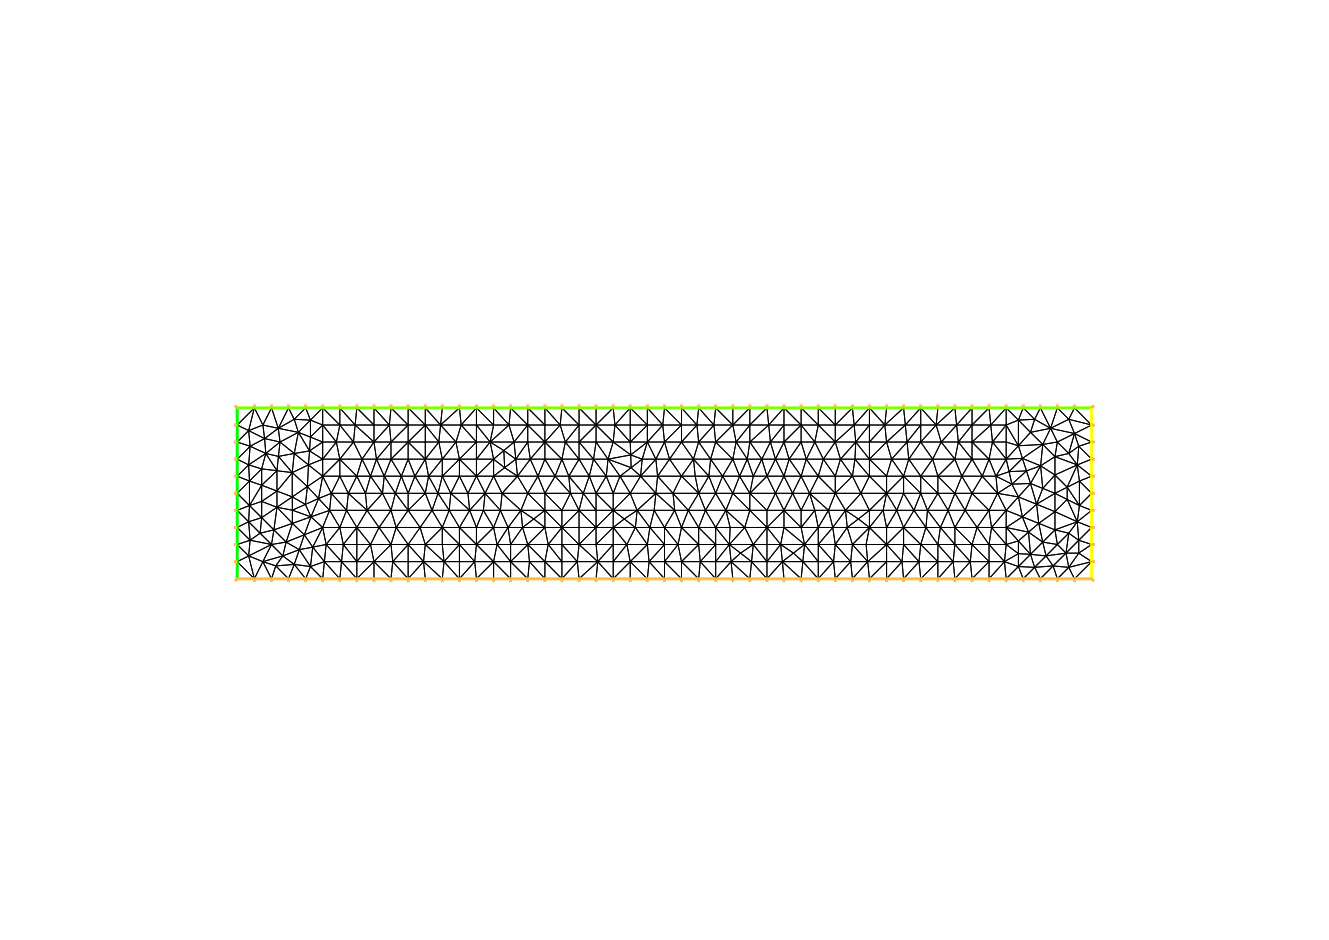
\includegraphics[width=.5\linewidth]{1}
		\caption{مرز ناحیه $\Omega$}
		%\label{fig:مرز ناحیه $\Omega$}
	\end{subfigure}%
	\begin{subfigure}{.5\textwidth}
		\centering
		
\includegraphics[width=.5\linewidth]{2}
		\caption{مثلث بندی ناحیه $\Omega$}
		%\label{fig مثلث بندی ناحیه $\Omega$}
	\end{subfigure}
	\caption{رسم ناحیه $\Omega$ و مثلث بندی آن}
	%\label{fig:رسم ناحیه $\Omega$ و مثلث بندی آن}
\end{figure}
 راه دیگر برای ساخت یک دامنه مربعی با مثلث بندی یکسان به صورت زیر است :
\begin{LTR}
	\begin{lstlisting}
 int m=3;
 int n=6;
 mesh Th = square (m ,n ,[x,y]) ; // build a square with m point on x direction and n point on y direction
 mesh Th1 = movemesh ( Th ,[x*2 ,y+1]) ; // translate the square [0 ,1]*[0 ,1] to a rectangle [0 ,2]*[1 ,2]
 savemesh ( Th1 ,"mesh.msh") ; // to save the mesh
 mesh Th2 ("mesh.msh") ; // to load the mesh
 plot(Th2);
	\end{lstlisting}
\end{LTR} 
نتیجه کد بالا به صورت زیر خواهد بود :
\begin{figure}[hbt!]
	\centering
	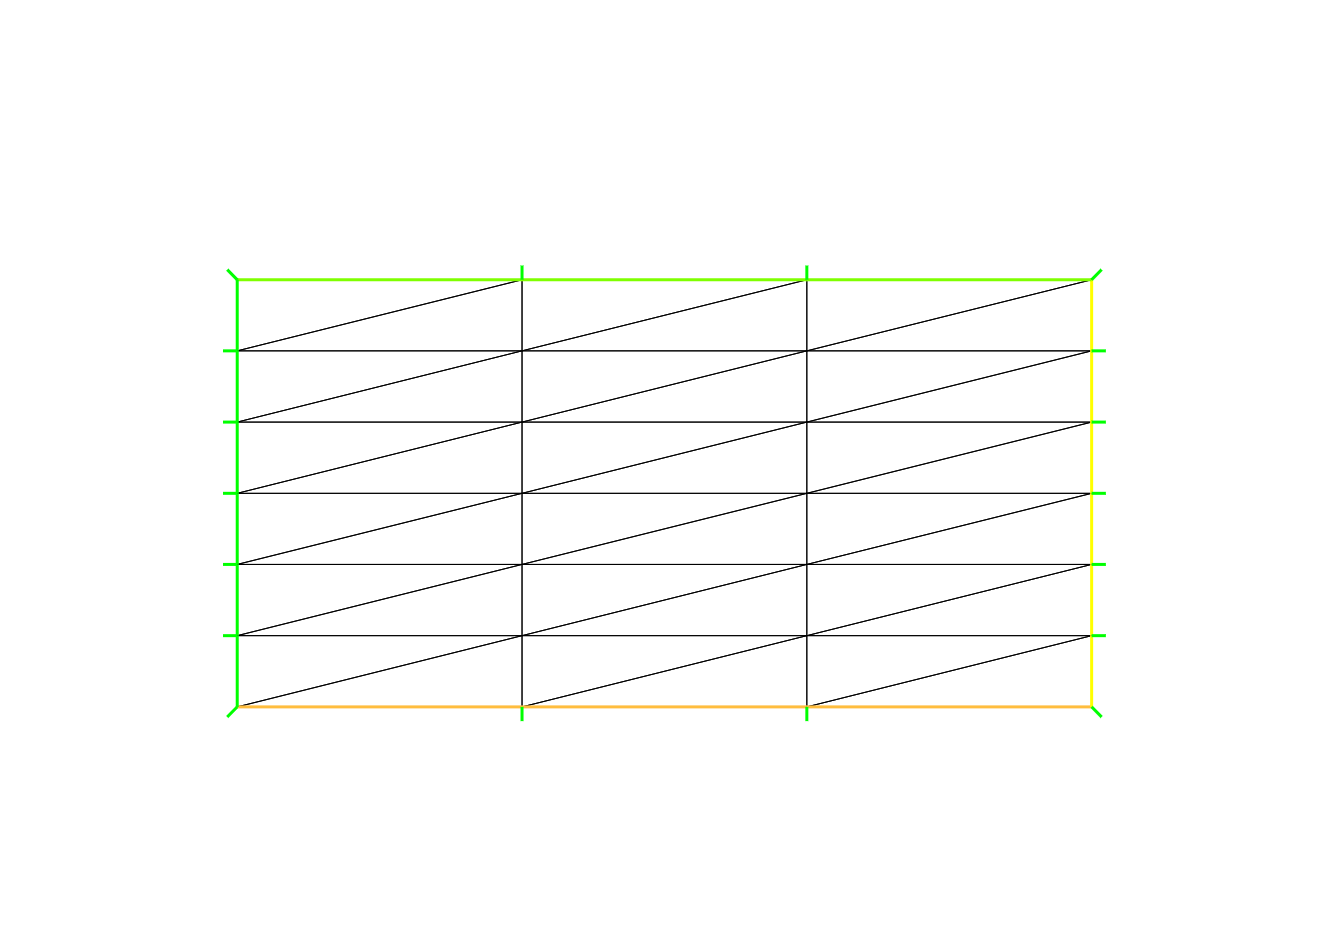
\includegraphics[width=\linewidth]{3}
	\caption{ ناحیه $\Omega$}
\end{figure}
همچنین ما می توانیم ناحیه خود را به صورت پارامتری تعریف کنیم :
\begin{LTR}
	\begin{lstlisting}
 border C(t = 0, 2*pi ){ x = cos(t); y = sin(t); label=1; }
 mesh Th = buildmesh(C(50)) ;
 plot(Th);
	\end{lstlisting}
\end{LTR} 
که نتیجه اش به صورت زیر خواهد بود :

\begin{figure}[hbt!]
	\centering
	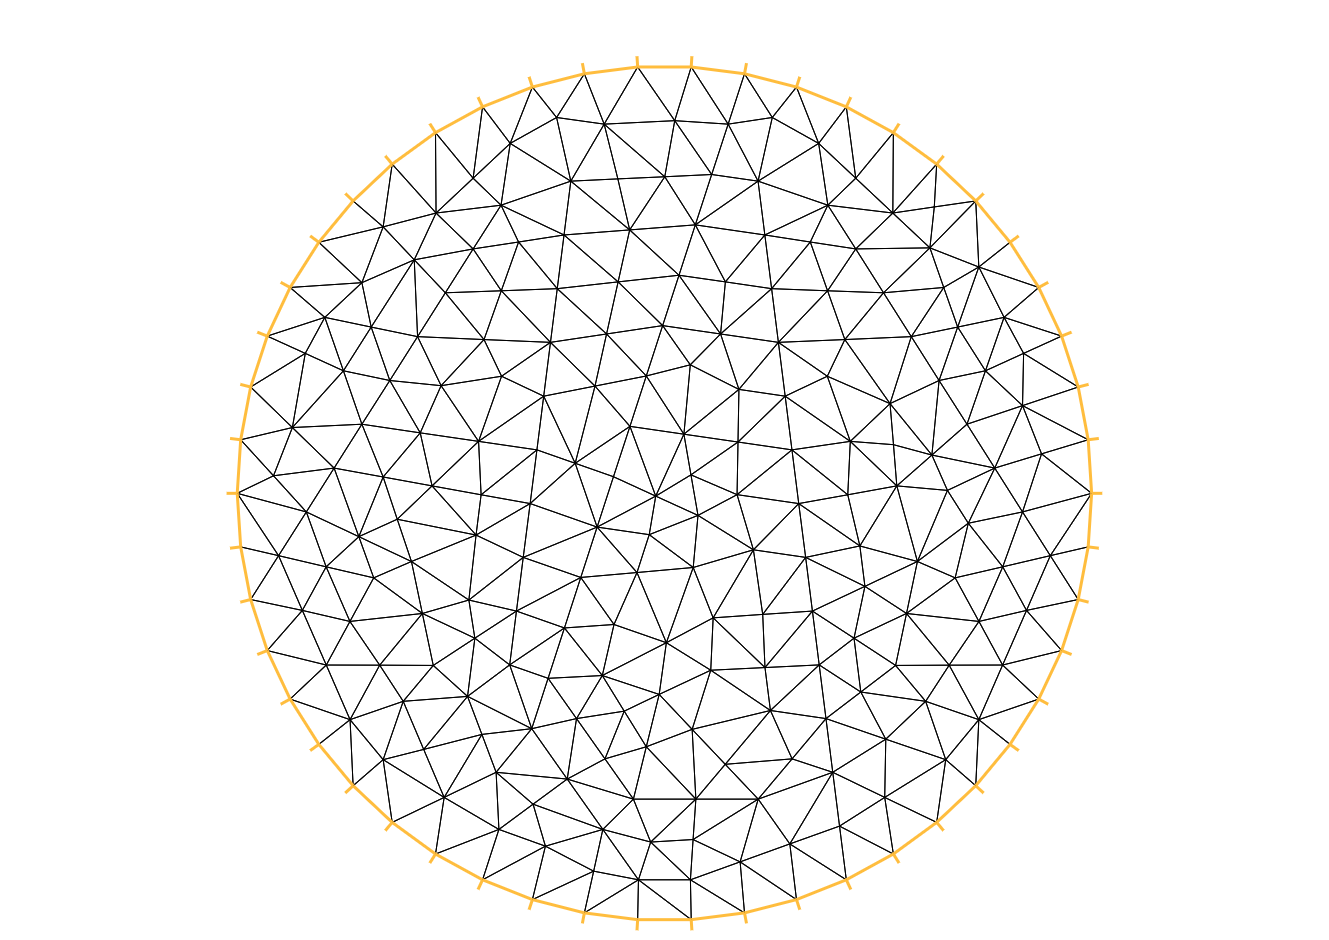
\includegraphics[width=\linewidth]{4}
	\caption{ تعریف ناحیه $\Omega$ به صورت پارامتری}
\end{figure}

\subsection{فضای عناصر متناهی}
عموما یک فضای عناصر متناهی عبارت است از فضای چندجمله ای های روی $T_{h}$ که دارای یک سری خواص معین باشند. ما یک فضای عناصر متناهی را به صورت 
\begin{LTR}
	\begin{lstlisting}
 fespace Vh ( Th , P1 ) ;
	\end{lstlisting}
\end{LTR}
تعریف می کنیم. تاکنون انواع فضاهای عناصر متناهی قابل دسترس عبارت اند از :
\begin{enumerate}
	\item P0
	\item  P03d
	\item  P1
	\item  P13d
	\item  P1dc
	\item  P1b
	\item  P1b3d
	\item  P2
	\item  P23d
	\item  P2b
	\item  P2dc
	\item  P3
	\item  P3dc
	\item  P4
	\item  P4dc
	\item  Morley
	\item  P2BR
	\item  RT0
	\item  RT03d
	\item  RT0Ortho
	\item  Edge03d
	\item  P1nc
	\item  RT1
	\item  RT1Ortho
	\item  BDM1
	\item  BDM1Ortho
	\item  TDNNS1
\end{enumerate}
که برای مثال P0 به صورت\\
$P0_{h} := \{ v \in L^{2}(\Omega) | \forall K \in T_{h} \exists \alpha_{K} \in \mathbb{R} : v|_{K} = \alpha_{K} \}$\\
تعریف می شود.
\subsection{شرایط مرزی}
برای تعریف شرط مرزی دیریکله روی مرز $ \Gamma_{d}  \subsetneq \mathbb{R} $ به صورت $u_{\Gamma_{d}} = f_{d}$ می توانیم به صورت on(gammad , u=f) عمل کنیم که u تابع مجهول است.
\section{حل مسئله}
ما روش های مختلف حل را برای معادله پواسون بررسی خواهیم کرد. این معادله به صورت زیر تعریف می شود: 
تابع $ u := \Omega \rightarrow \mathbb{R} $ را چنان بیابید که برای تابع $f\in L^{2}(\Omega)$ داده شده را چنان بیابید که در\\



\[   
\begin{cases}
-\bigtriangleup u=f &\quad\text{in } \Omega\\
u = 0 &\quad\text{on } \partial \Omega\\ 
\end{cases}
\]\\
صدق کند. فرم تغییراتی این مسئله به صورت یافتن $u \in H^{1}_{0}(\Omega)$ به قسمی که به ازای هر $v \in H^{1}_{0}(\Omega)$ تساوی\\ 
\[   
a(u,v) = l(v) 
\]\\
که در آن
\[
\begin{cases}   
a(u,v) = \int_{\Omega} \bigtriangledown u \cdot \bigtriangledown v dxdy\\
l(v) = \int_{\Omega} f \cdot v dxdy
\end{cases}
\]\\
است نوشته می شود.\\
حال فرض کنیم $T_{h}$ یک مثلث بندی هموار از $\Omega$ با مثلث های از اندازه حداکثر $h<1$ باشد. همچنین فرض کنیم \\
\[
V_{h} := \{ v_{h} \in C^{0}(\bar{\Omega}); v_{h}|_{T} \in \mathbb{P}_{1}(T) , \forall T \in T_{h}; v_{h} = 0 \text{on }\partial\Omega \}
\]\\
یک زیر فضای عناصر متناهی از $ H^{1}_{0}(\Omega)$ است و $\mathbb{P}_{1}$ مجموعه چندجمله ای های درجه کمتر یا مساوی یک روی $\mathbb{R}$ است و بنابراین فرم ضعیف معادله پواسون عبارت است از پیدا کردن $u_{h} \in V_{h}$ به قسمی که به ازای هر $v_{h} \in V_{h}$ در معادله\\
\[   
\int_{\Omega} \bigtriangledown u_{h} \cdot \bigtriangledown v_{h} dxdy - \int_{\Omega} f \cdot v_{h} dxdy = 0
\]\\
صدق کند.
\subsection{دستور solve}
اولین شیوه حل معادله، تعریف و حل به صورت هم زمان به صورت زیر است.
\begin{LTR}
	\begin{lstlisting}
 solve poisson ( uh , vh , init =i, solver = LU ) = // Solve Poisson Equation
	int2d ( Th ) ( Grad ( uh ) ’* Grad ( vh ) ) // bilinear form
	-int2d ( Th ) ( f * vh ) // linear form
	+on (1 ,2 ,3 ,4 , uh =0) ; // Dirichlet B.C.
	\end{lstlisting}
\end{LTR}
\subsection{دستور problem}
در این روش ابتدا مسئله را با دستور problem تعریف و سپس با فراخوانی نام تخصیص داده شده به حل آن اقدام می کنیم.
\begin{LTR}
	\begin{lstlisting}
 problem poisson (uh , vh , init =i, solver = LU ) =// Definition of the problem
	int2d ( Th ) ( Grad ( uh ) ’* Grad ( vh ) ) // bilinear form
	-int2d ( Th ) ( f * vh ) // linear form
	+on (1 ,2 ,3 ,4 , uh =0) ; // Dirichlet B.C.
 Poisson ; // Solve Poisson Equation
	\end{lstlisting}
\end{LTR}


%\chapter{...}
\begin{LTR}
	\begin{algorithm}[H]
		\KwData{inputs}
		\KwResult{outputs}
		initialization\;
		\While{condition}{
			do something\;
		}
		\caption{algorithm skeleton}
	\end{algorithm}
	\begin{center}
		\begin{table}[]
			\centering
			\begin{tabular}{ l | c | r }		
				& 0 & 1 \\
				\hline	
				0 & 0 & 1 \\
				1 & 1 & 10 \\
				\hline  
			\end{tabular}
			\caption{جمع باینری}
		\end{table}
	\end{center}
\end{LTR}

%\begin{thebibliography}{99} % assumes less than 100 references
\addcontentsline{toc}{section}{Refrences} % to add the references to index
\begin{LTR}
\bibitem{baseArticle}
Khoo, Yuehaw, Jianfeng Lu and L. I. U. Ying. “Solving PDE problems with uncertainty using neural-networks.” (2018).

\bibitem{UQIntro}
Sullivan, Timothy John. Introduction to uncertainty quantification. Vol. 63. Springer, 2015.
\end{LTR}

%چنانچه مرجع فارسی نیز داشته باشید باید دستور فوق را فعال کنید و مراجع فارسی خود را بعد از این دستور وارد کنید



\end{thebibliography}

%--------------------------------------------------------------------------------------------------------
% -------------------- DON'T EDIT ----------------------------------------
% the following lines are needed for making the appendixes name correct in the index.
\makeatletter
\def\@makechapterhead#1{%
  \vspace*{50\p@}%
  {\parindent \z@ \centering\normalfont
    \ifnum \c@secnumdepth >\m@ne
      \if@mainmatter
        \huge\bfseries \@chapapp\space \thechapter
        \par\nobreak
        \vskip 20\p@
      \fi
    \fi
    \interlinepenalty\@M
    \Huge \bfseries #1\par\nobreak
    \vskip 40\p@  }}
%--------------------------------------------------------------------------------------------------------
% -------------------- Please EDIT ----------------------------------------

%\appendix
%\chapter{عنوان فصل یا پیوست}
متن فصل را در اینجا بنویسید.

\section{عنوان بخش }
متن بخش را می توانید در این ناحیه بنویسید.

\subsection{عنوان زیر بخش }
متن زیر بخش را می توانید در این قسمت بنویسید 
%\chapter{عنوان فصل یا پیوست}
متن فصل را در اینجا بنویسید.

\section{عنوان بخش }
متن بخش را می توانید در این ناحیه بنویسید.

\subsection{عنوان زیر بخش }
متن زیر بخش را می توانید در این قسمت بنویسید

%\bibliographystyle{unsrt-fa}
% اگر فایل bibtex با پسوند bib حاوی اطلاعات مربوط به مراجع خود با فرمت صحیح bibtex را دارید از خط زیر استفاده کنید و به جای MyReferences نامه فایل خود را بنویسید.

% در این نمونه پایان‌نامه فرض شده است که شما فایل bib حاوی اطلاعات مربوط به مراجع خود با نام MyReferences.bib را دارید.
%\bibliography{MyReferences}
%\nocite{semiconcave}

% اگر به صورت عادی می‌خواهید ارجاع دهید خط بالا را غیر فعال کرده و قسمت زیر را فعال کنید و طبق مثال عمل کنید (البته این روش حرفه‌ای نیست و توصیه نمی‌شود).
%\begin{thebibliography}{9}
%\begin{latin}
%	content...

%\end{latin}
%\end{thebibliography}

   %
   % در صورتی که می‌خواهید عنوان «واژه‌نامه فارسی به انگلیسی» در فهرست مطالب 
   % وارد شود، علامت «%» را از ابتدای خط زیر حذف کنید.
\addcontentsline{toc}{section}{واژه‌نامه فارسی به انگلیسی }

\begin{center}
\vspace{1.5cm}
\Huge{واژه‌نامه فارسی به انگلیسی}
\vspace{1.5cm}
\end{center}
%\begin{center}
%الف
                     
%\end{center}
\begin{RTL}
	% \dotfill\lr{‌open source}\\
	شبکه عصبی پیچشی                              \dotfill               \lr{convolutional neural-network}                       \\
	یادگیری عمیق                              \dotfill               \lr{‌deep learning}                       \\
	روش تفاضلات متناهی                              \dotfill               \lr{‌finite difference method}                       \\
	روش عناصر متناهی                              \dotfill               \lr{‌finite element method}                       \\
	محیط ناهمگن                              \dotfill               \lr{‌inhomogeneous media}                       \\
		شبکه عصبی                              \dotfill               \lr{‌neural-network}                       \\
			بعد فضائی                              \dotfill               \lr{‌spatial dimension}                       \\
				عدم قطعیت                              \dotfill               \lr{‌uncertainty}                       \\
					مقدار سنجی عدم قطعیت                              \dotfill               \lr{‌uncertainty quantification}                       \\
					غیر خطی \dotfill \lr{nonlinear}\\
					مشتق‌گیری اتوماتیک \dotfill \lr{automatic differentiation} \\
					هسته پردازنده گرافیکی \dotfill \lr{graphic processor unit (GPU)} \\
					شبکه رو به جلو \dotfill \lr{feedforward neural network} \\
					شبکه عصبی مصنوعی \dotfill \lr{artificial neural network} \\
					بایاس \dotfill \lr{bias} \\
					وزن \dotfill \lr{weight} \\
					تابع فعال‌سازی \dotfill \lr{activation function} \\
					تابع هزینه \dotfill \lr{loss function} \\
					نورون \dotfill \lr{neuron} \\
					پایگاه داده مستخرج از یک منبع \dotfill \lr{dataset} \\
					پایگاه داده مستخرج از منابع متفاوت \dotfill \lr{data set} \\
					بیش همسان سازی \dotfill \lr{overfitting} \\
					کم همسان سازی \dotfill \lr{underfitting} \\
					گشت در داده ها \dotfill \lr{epoch} \\
					دسته \dotfill \lr{batch} \\
					روش کاهش آشوبناک گرادیان \dotfill \lr{stochastic gradient decent (SGD)} \\
					
							
\end{RTL} % include persian to english dictionary

% --------------------------------------   INFORMATION IN LATIN  ----------------------------------------------
%\begin{latin}
%\latintitle{FreeFem++, a tool to solve PDEs numerically}
%\latinauthor{Sajed N. Zarin pour}
% --------------------------------------
% choose and activate one of the following lines
%\latindegree{Master's Thesis}
%\latindegree{Ph.D. Thesis}
% --------------------------------------
%\latinthesisdate{March 2019}
%\latinsupervisor{Dr. Khadije A. Nedaii}
% If you have advisor, write its name in the following line, otherwise inactive (comment) the line.
%\latinadvisor{Name of Advisor} \advisorexisttrue
%\latindepartment{Mathematics}
%\latinuniversity{Institute for Advanced Studies in Basic Sciences}
%\latincity{Zanjan}
%\begin{latinabstract}
%\noindent 
Towards modeling the real-world phenomenons with partial differential equations that involve uncertainties, one of the major difficulties that show itself is the curse of dimensionality. We encounter that when we was going to model soft tissue deformation using finite element method. Luckily, very often the variability of physical quantities derived from the model can be captured by a few features on the coefficient fields. On the other hand, nowadays, it had seen that the marriage between neural-networks and numerical methods is very fruitful. For example, one can use neural-networks based methods to parametrize the physical quantity of interest as a function of input coefficients; In that case, the representability of such quantity can be justified by viewing the neural-networks as performing time evolution to find the solution to the model, as indeed, in this thesis we would like to study the use of neural-networks on two notable partial differential equations in engineering and physics to that end. Furthermore, we would like to try to find an answer to this question: How simplicity and accuracy are tradings when we use neural-networks?

\latinkeywords{Partial Differential Equations,Finite Element Method, Uncertainty Quantification}

%\end{latinabstract}
%\makelatintitle
%\end{latin}

\end{document}
